\documentclass[table,aspectratio=169]{beamer}

\usefonttheme{professionalfonts}
\usefonttheme[onlymath]{serif}

\mode<presentation>
{
\usetheme{CambridgeUS}
\setbeamercolor{item projected}{bg=darkred}
\setbeamertemplate{enumerate items}[default]
\setbeamertemplate{navigation symbols}{}
\setbeamertemplate{itemize item}{-}
\setbeamertemplate{itemize subitem}[triangle]
\setbeamercovered{transparent}
\setbeamercolor{block title}{fg=darkred}
\setbeamercolor{local structure}{parent=alerted text}
}
\addtobeamertemplate{block begin}{\setbeamercolor{local structure}{parent=structure}}{}

\usepackage[english]{babel}
\usepackage{amssymb}
\usepackage{mathcmd}
\usepackage{nicefrac}
\usepackage{booktabs}
\usepackage{graphicx}
\usepackage{siunitx}
\usepackage{bbm}
\usepackage{url}
\usepackage{acronym}
\graphicspath{{./}{./../talk_plots/}{./../talk_figures/}{./../../plots/}}

%\usepackage{courier}
%\usepackage{times}
% The non-standard packages arev and bera define fonts which look nicely for
% projection, you might want to try them instead of Times/Helvetica/Courier.
% Use the

\acrodef{ICAO}{International Civil Aviation Organization}

%%%%%%%%%%%%%%%%%%%%%%%%%%%%%%%%%%%%%%%%%%%%%%%%%%%%%%%%%%%%%%%%%%%%%%%%
\usepackage{pxfonts} % Or palatino or mathpazo
\usepackage{eulervm}
\linespread{1.05}
%%%%%%%%%%%%%%%%%%%%%%%%%%%%%%%%%%%%%%%%%%%%%%%%%%%%%%%%%%%%%%%%%%%%%%%%
\usepackage[T1]{fontenc}
% Or whatever. Note that the encoding and the font should match. If T1
% does not look nice, try deleting the line with the fontenc.
\usepackage{hyperref}

\newcommand{\prob}[1]{\ensuremath{\mathbb{P}\left(  #1 \right)}}
\newcommand{\mean}[1]{\ensuremath{\mathbb{E}\left(  #1 \right)}}
\newcommand\independent{\protect\mathpalette{\protect\independenT}{\perp}}
\newcommand{\menquote}[1]{\ensuremath{\text{\textquotedbl} #1 \text{\textquotedbl}}}
\def\independenT#1#2{\mathrel{\rlap{\(#1#2\)}\mkern2mu{#1#2}}}

\definecolor{eham}{rgb}{1.0, 0.714, 0.467}
\definecolor{egll}{rgb}{0.427, 0.714, 1.0}
\definecolor{egss}{rgb}{0.859, 0.82, 0.0}
\definecolor{lgav}{rgb}{0.0, 0.427, 0.859}
\definecolor{lemd}{rgb}{0.573, 0.0, 0.0}
\definecolor{egkk}{rgb}{0.0, 0.286, 0.286}
\definecolor{lirf}{rgb}{0.141, 1.0, 0.141}
\definecolor{eddf}{rgb}{0.286, 0.0, 0.573}
\definecolor{eggw}{rgb}{0.714, 0.859, 1.0}
\definecolor{lfpg}{rgb}{0.573, 0.286, 0.0}

\newcommand{\airp}[1]{\textcolor{#1}{\textsc{#1}}}


%\setbeamerfont{alerted text}{series=\scshape}

\title[Pre-Scheduled Random Arrivals]
{Pre-Scheduled Random Arrivals for modelling air traffic operations}
\subtitle{Analytical and applied results}

\author[Carlo Lancia]{Carlo Lancia}

\institute[Leiden Univ.]{Mathematical Institute Leiden University}

\date[TU Delft Prob \& Stats Seminar]{TU Delft, October 16, 2017\\Seminar Series in Probability and Statistics}
% - Either use conference name or its abbreviation.
% - Not really informative to the audience, more for people (including
%   yourself) who are reading the slides online

% \usepackage{hyperref}
% \subject{Cutoff phenomenon for finite Markov chains}
% This is only inserted into the PDF information catalog. Can be left
% out.

% \AtBeginSection[]
% {
%   \begin{frame}<beamer>
%     \frametitle{Outline}
%     \tableofcontents[currentsection,hideothersubsections]
%   \end{frame}
% }
% Use this if you do want the table of contents to pop up at
% the beginning of each subsection.

% \pgfdeclareimage[height=2em,interpolate=true]{ntnulogotext}{foo}
% If you want to include a different logo on the title page
% only (e.g. a combined logo of different institutions), you
% can use this command.

% -------------------------------------
% \includeonlyframes{current}
% -------------------------------------

\begin{document}

\maketitle
% You can use \maketitle to create the titlepage,
% or \compressedtitle to create a more compact titlepage
% with the look of the other pages in compress style

% \begin{frame}
%   \titlepage
% \end{frame}
% Or you can call the titlepage command in a frame environment

\begin{frame}<beamer>[label=current]
    \frametitle{Outline}
    \tableofcontents[hideallsubsections]
\end{frame}

\section{Introduction}

\begin{frame}[t]\frametitle{Pre-Scheduled Random Arrivals (PSRA)}
    \begin{itemize}
        \item Continuous-time point process of the form
        \[t_i = \nicefrac{i}{\lambda} + \xi_i\]
        \item $\lambda$ is a fixed constant
        \item $\{\xi_i\}_i$ is a sequence of i.i.d.\ random variables
        \item Optional \emph{thinning} of intensity $\rho$ (later)
    \end{itemize}
    \vfill
    \centering
    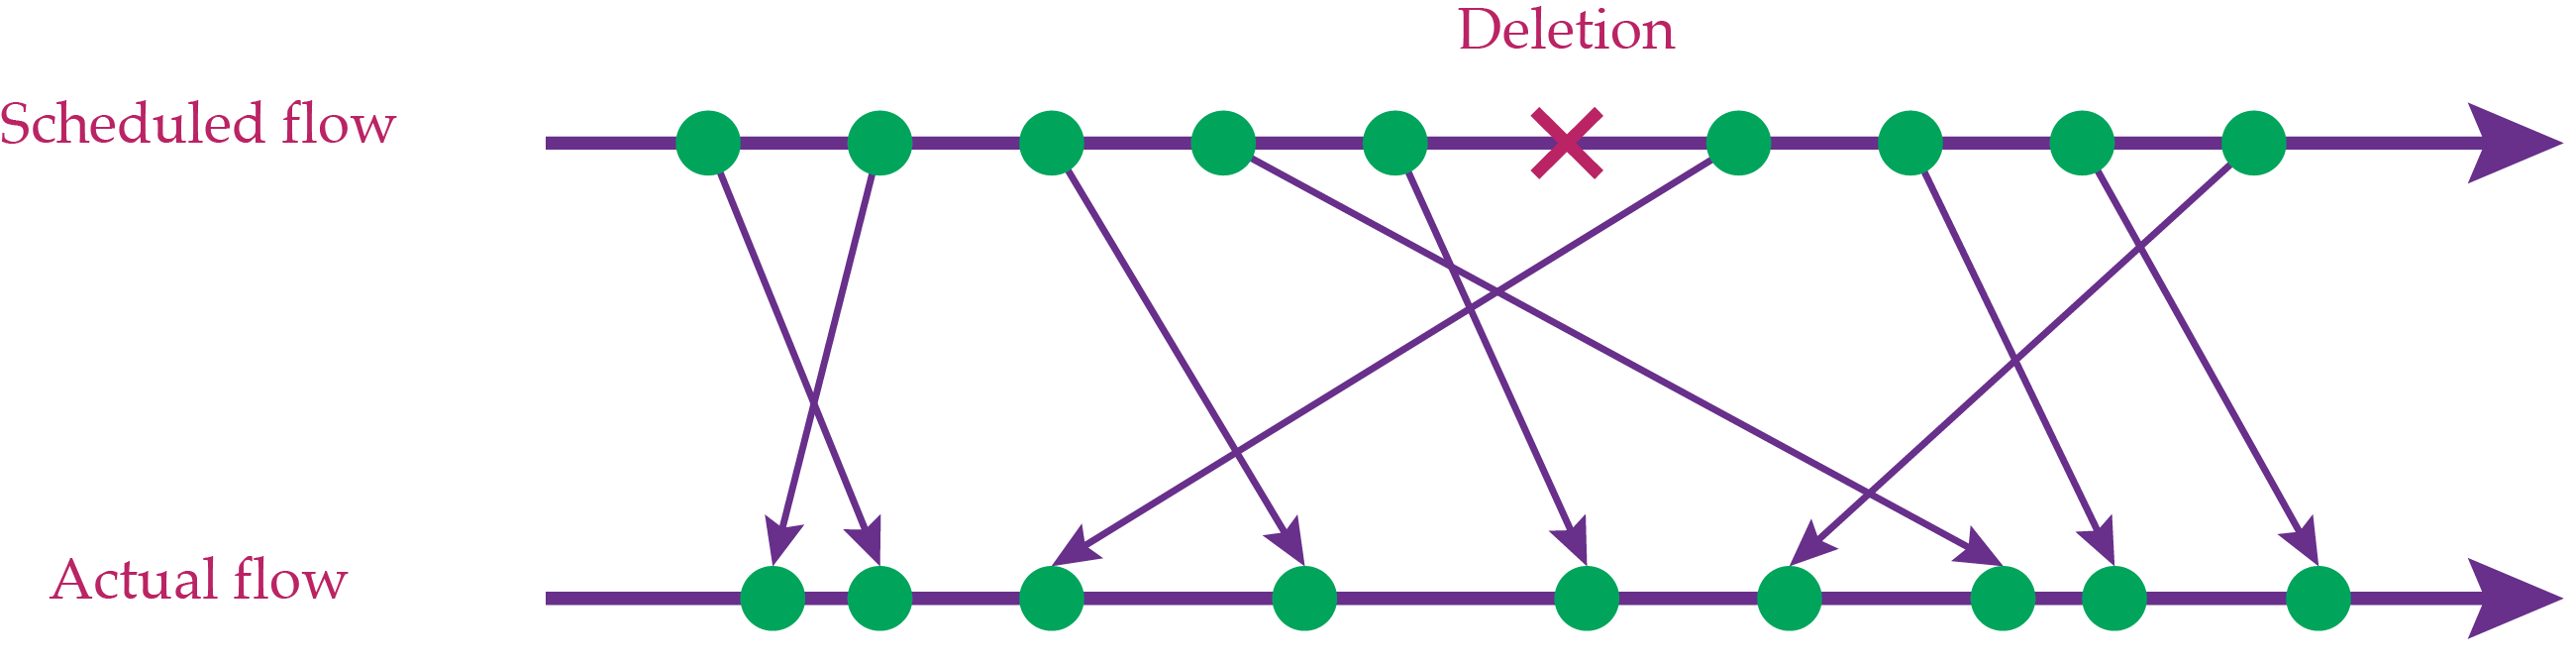
\includegraphics[width= 0.9\textwidth]{psra-1}
\end{frame}

\begin{frame}[t]\frametitle{Range of applications}
    \begin{itemize}
        \item Public transportation systems
        \item Vessels marine traffic
        \item Crane handling in loading/unloading operations
        \item Outpatient scheduling
    \end{itemize}

    \vfill

    \begin{center}
        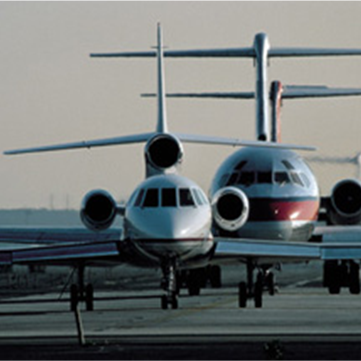
\includegraphics[width=.18\textwidth]{air-transport}
        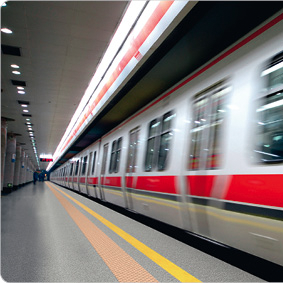
\includegraphics[width=.18\textwidth]{railways}
        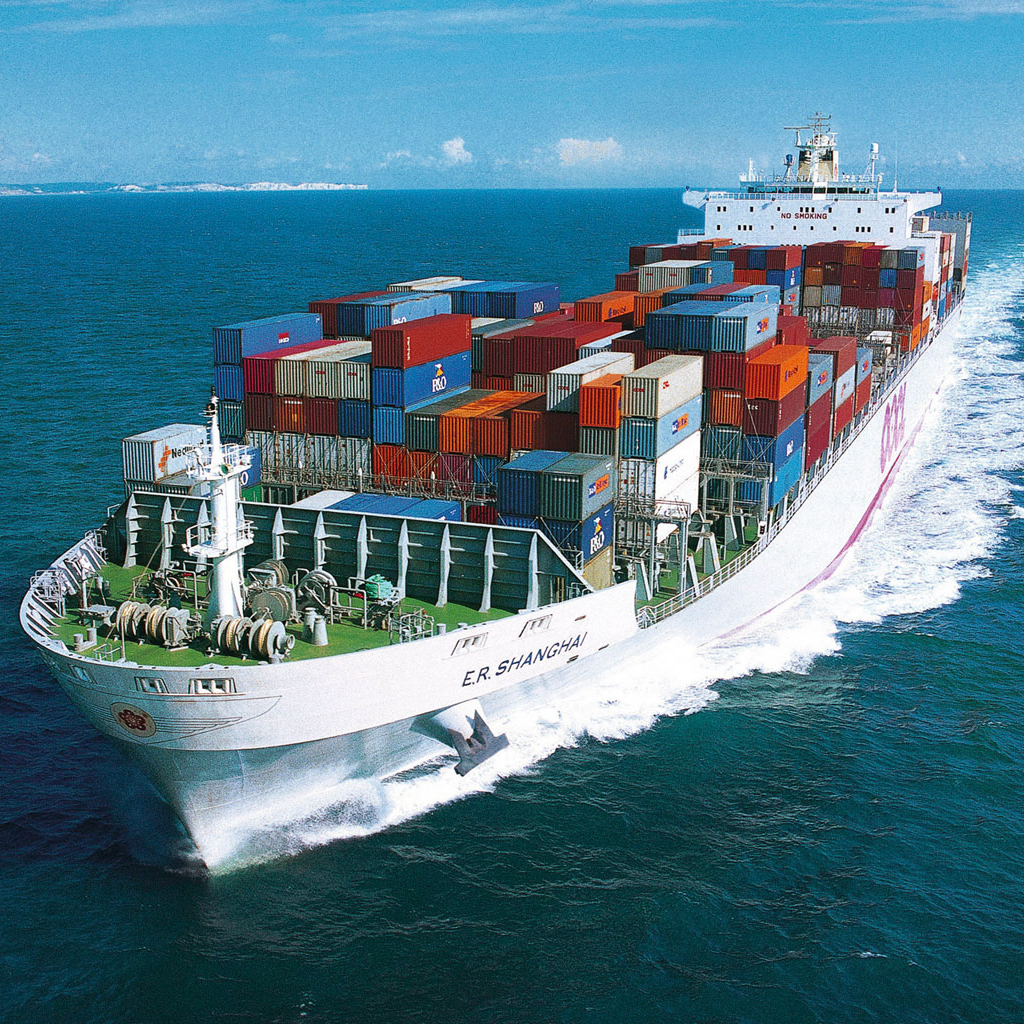
\includegraphics[width=.18\textwidth]{vessel}
        \includegraphics[width=.18\textwidth]{crane}
        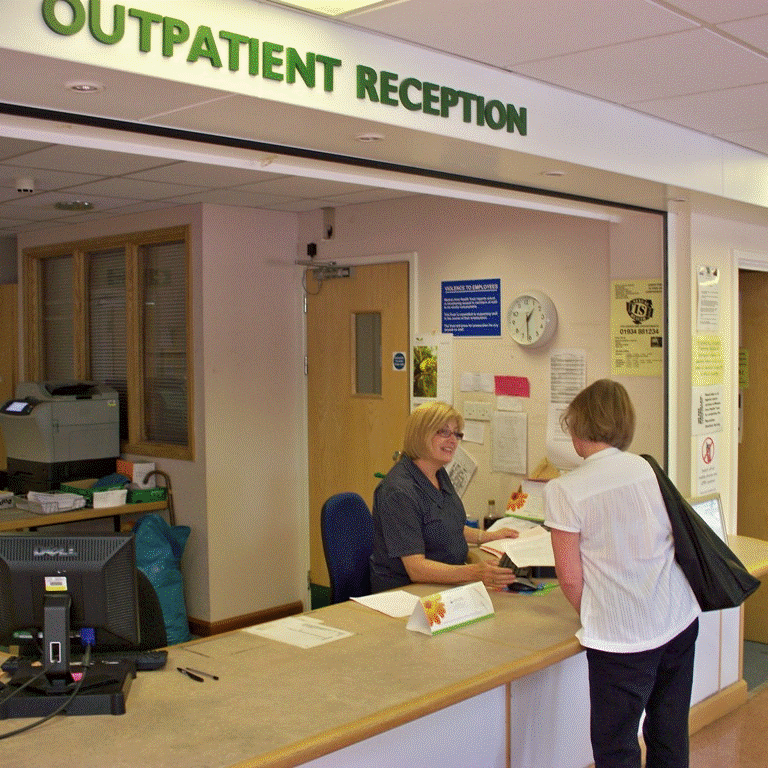
\includegraphics[width=.18\textwidth]{outpatient}
    \end{center}

    \vfill

    \alert{All systems where scheduled arrivals are intrinsically subject to
    random variations.}
\end{frame}

\begin{frame}[t]\frametitle{Properties of PSRA}
    \[t_i = \nicefrac{i}{\lambda} + \xi_i\]
    \begin{itemize}
        \item We usually require $\mathbb{E}(\xi_i) = 0$ and $\sigma(\xi_i) < \infty$
        \item Interpretation as a random translation of the integers $z\in\mathbb{Z}$ (1D crystal)
        \item Weak convergence to the Poisson process for $\sigma \to \infty$ (1D gas)
        \item If $N_1$ and $N_2$ are the number of arrivals in $(t,t+T]$ and $(t + T , t + 2T ]$ then
        $\text{Cov}(N_1,N_2)<0$
        \item A congested period is likely to be followed
        by one with less arrivals than expected
    \end{itemize}
\end{frame}

\section{A queue model for Heathrow airport}

\begin{frame}[t]\frametitle{London Heathrow Airport}
    \begin{columns}
        \column{.5\textwidth}
        \begin{itemize}
            \item Second busiest airport in the world by international passenger traffic
            \item Busiest airport in Europe by passenger traffic (both transit and terminal)
            \item Seventh busiest airport in the world by total passenger traffic (enplaned, deplaned, and direct-transit)
            \item 75.7 million passengers in 2016 (+1.0\% increase from 2015)
        \end{itemize}
        \column{.5\textwidth}
        \centering
        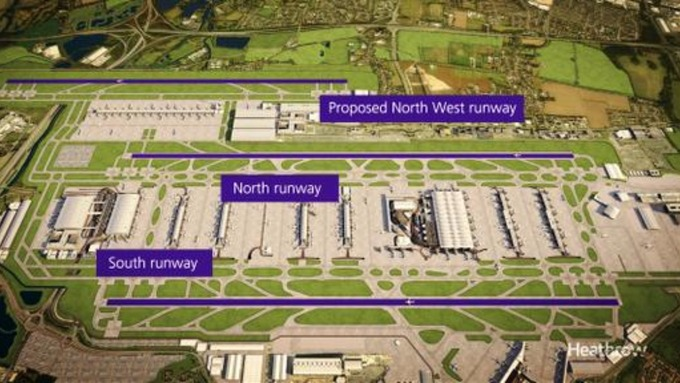
\includegraphics[width=.95\textwidth]{stream_img}
        {\small \url{http://news.images.itv.com/image/file/704067/stream_img.jpg}}
    \end{columns}
\end{frame}

\begin{frame}[t]\frametitle{PSRA/D/1}
    \centering
    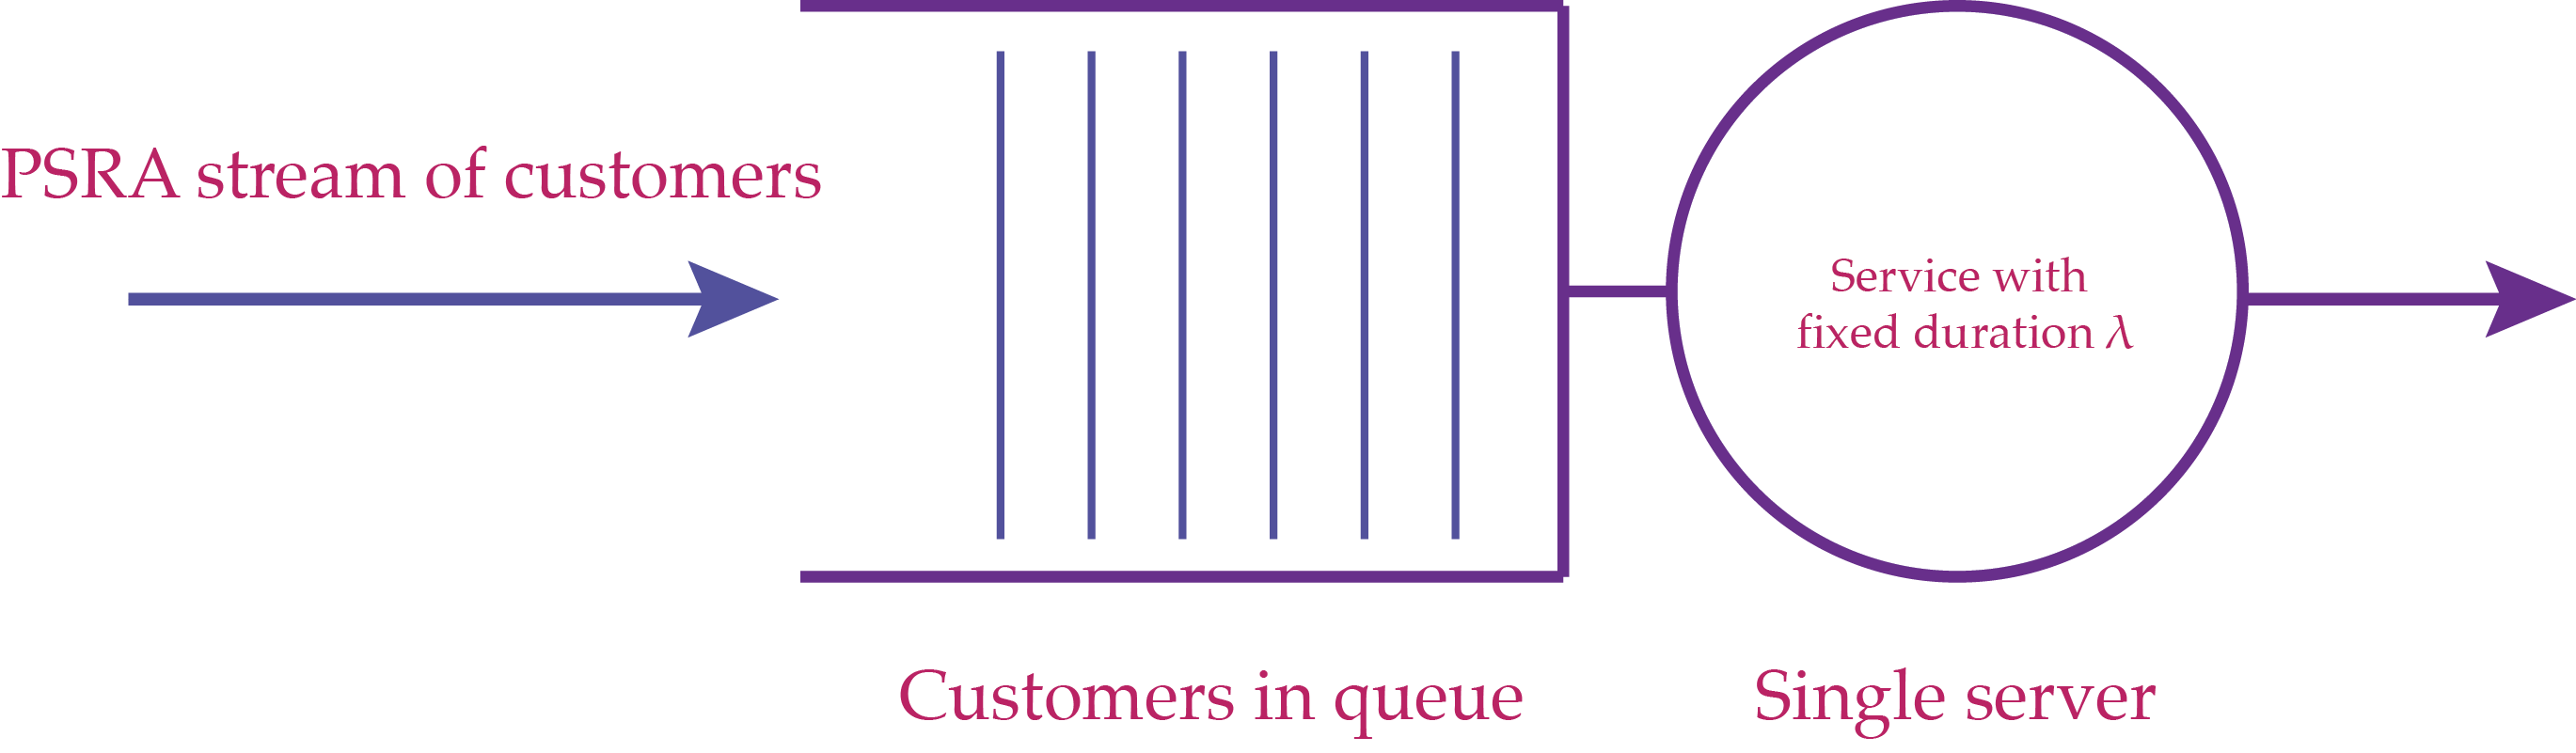
\includegraphics[width= .6\textwidth]{psra-d-1}
    \vfill
    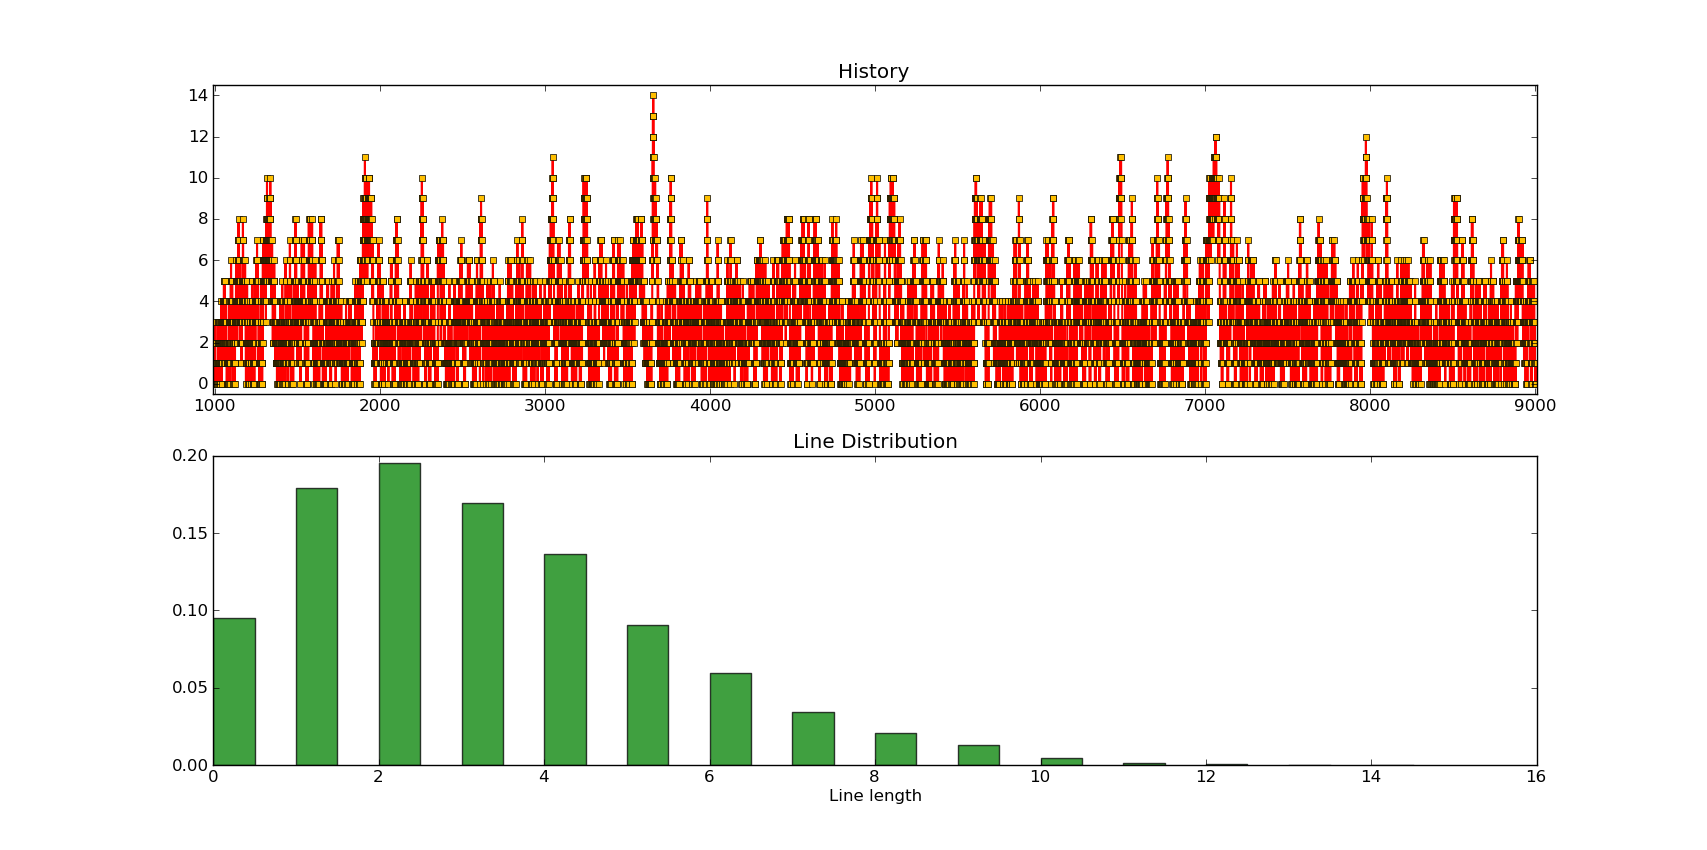
\includegraphics[width=.6\textwidth]{U10D}
\end{frame}

\begin{frame}{Insensitivity to the delays law with fixed $\sigma$}
    \centering
    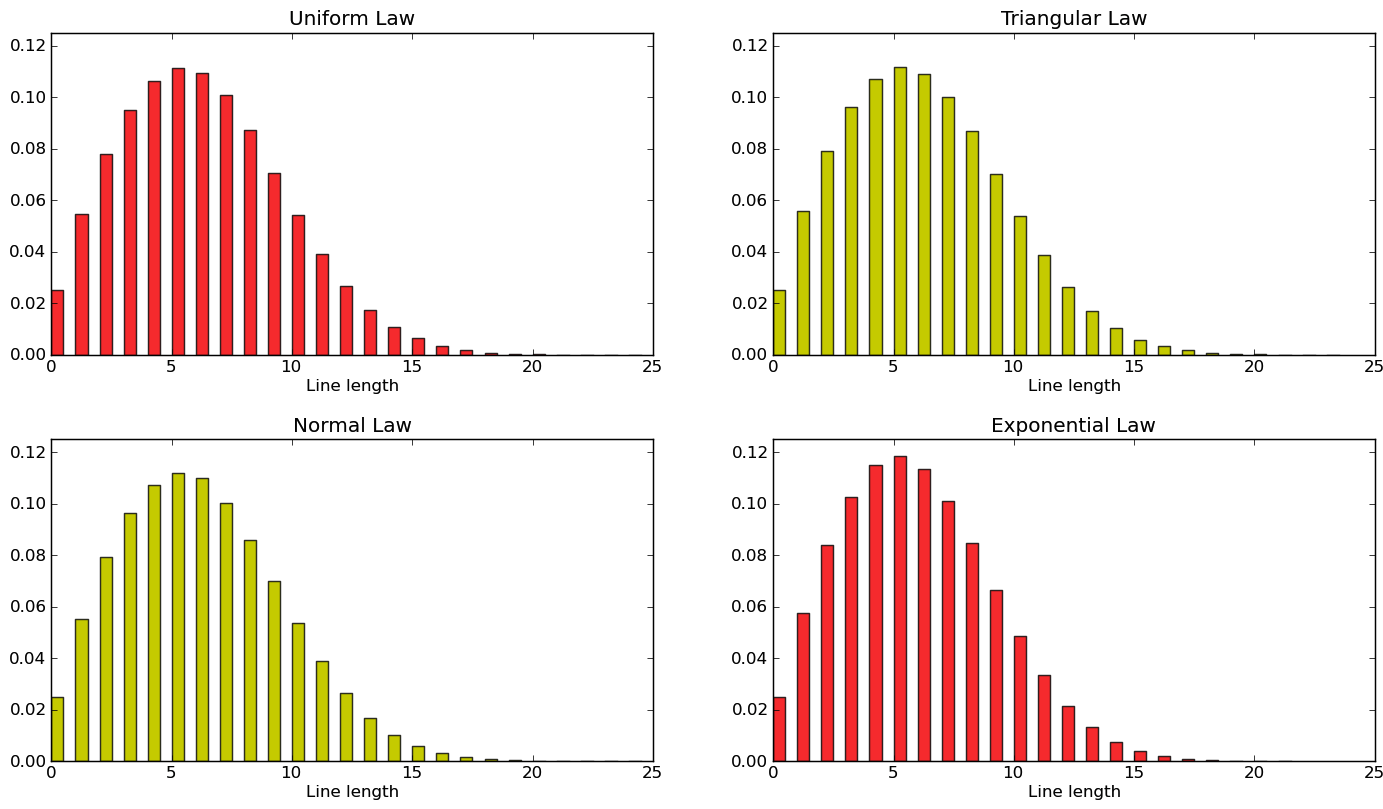
\includegraphics[width=.75\textwidth]{insensitiveness}
\end{frame}

\begin{frame}[t]\frametitle{PSRA/D/1 vs M/D/1}
    \begin{itemize}
        \item Poisson arrivals (M) are the \emph{golden stardard}
        in the Air Traffic Management domain
        \item PSRA thinned with intensity $\rho = \frac{40}{41}$
        \item Uniform delays with $\sigma = \nicefrac{20}{\lambda} = 30$ min
        \item Service parameter for both models is $\rho$
    \end{itemize}
    \centering
    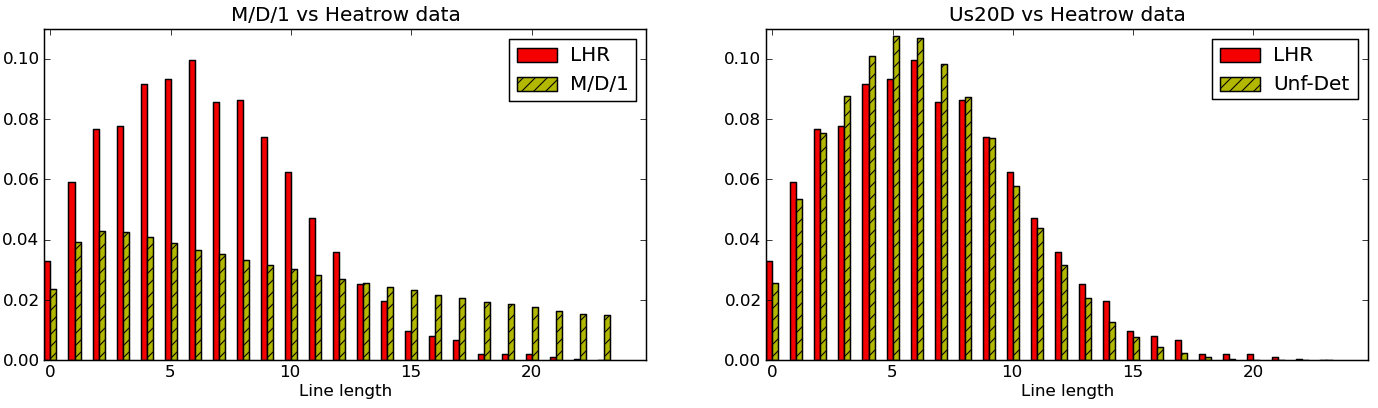
\includegraphics[width=\textwidth]{cills}
\end{frame}

\begin{frame}[t]\frametitle{Limitations}
    \begin{columns}
        \column{.6\textwidth}
        \begin{center}
            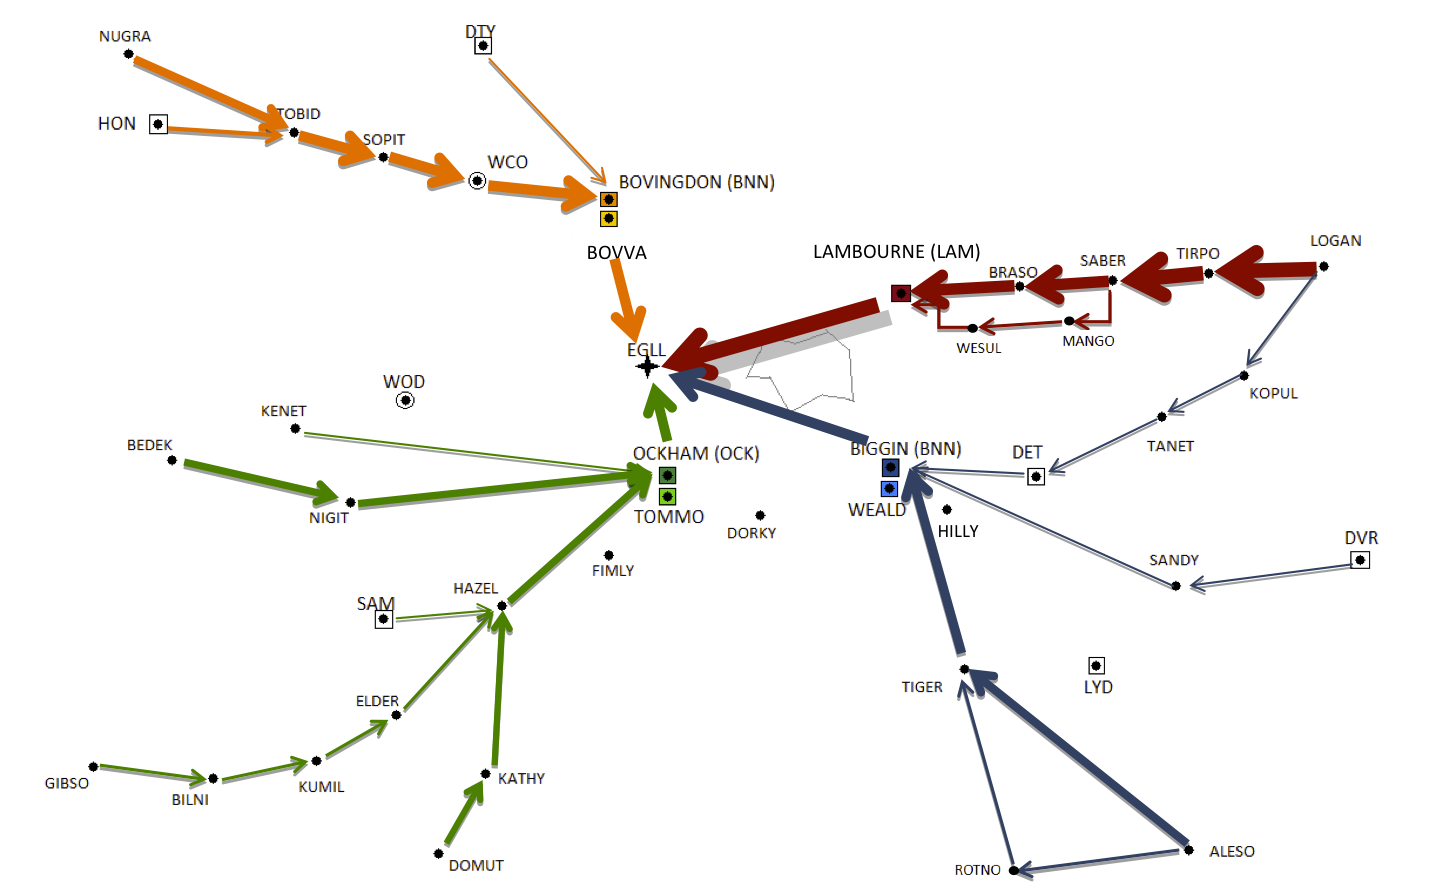
\includegraphics[width=.85\textwidth]{cills2}

            {\tiny From Caccavale et al. (2014) \emph{J Air Transp Manag}, 34, 116--122}
        \end{center}
        \column{.4\textwidth}
        \begin{itemize}
            % \item Indirect comparison with Poisson, i.e.\ through a queueing model
            \item Indirect comparison through a \alert{$\cdot$/D/1 queue model}
            \item Analysis overlooks action of Traffic Control
            \item \emph{This leads to overestimating PSRA parameter $\sigma$}
            \item Deterministic schedule of PSRA is equally spaced in time (OK for Heathrow, though)
        \end{itemize}
    \end{columns}
\end{frame}


\section{Inbound flow at some major European airports}

% \begin{frame}[t]\frametitle{Summary}
%     \begin{alertblock}{Problem}
%         Estimating the daily demand at major European airports
%     \end{alertblock}
%
%     \begin{alertblock}{Data and Methods}
%         \begin{itemize}
%             \item Entrance time in a cylinder of radius 40 NM around airport
%             \item Data-driven definition of Poisson process and Pre-scheduled Random Arrivals
%             \item Comparison of the two processes
%         \end{itemize}
%     \end{alertblock}
%
%     \begin{alertblock}{Conclusions}
%         PSRA outperforms Poisson arrivals in estimating the daily demand
%     \end{alertblock}
% \end{frame}

%
\begin{frame}[t]\frametitle{Airport selection and Arrival areas}
    \centering
    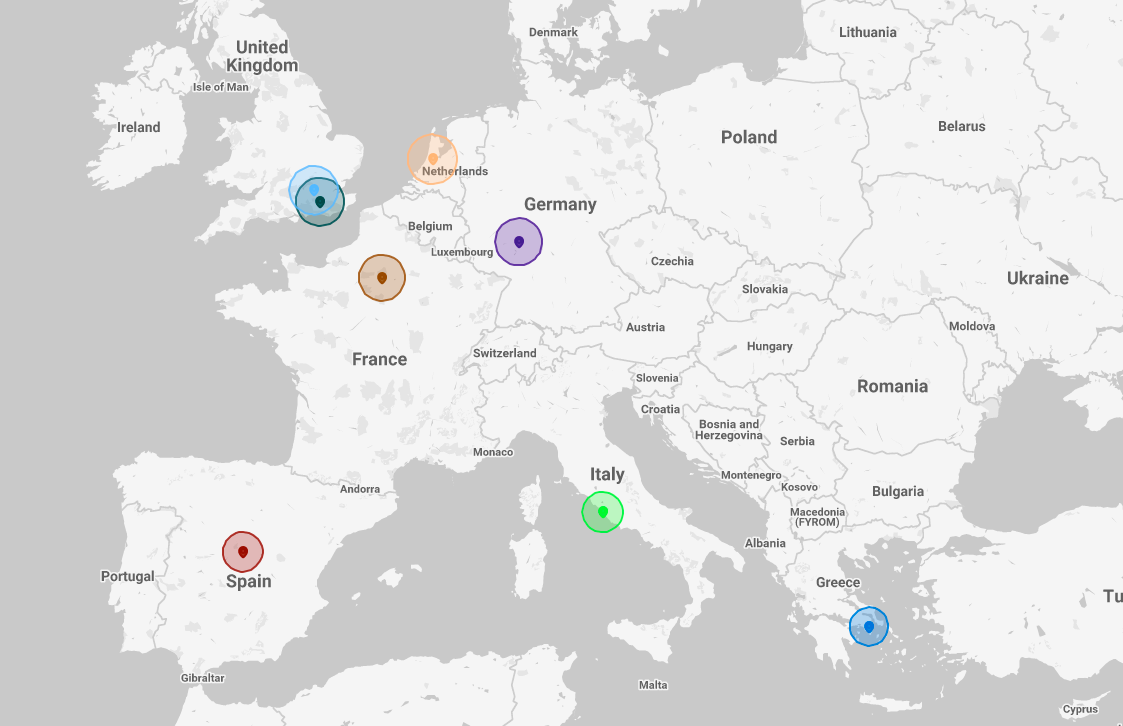
\includegraphics[width=.7\textwidth]{map}
\end{frame}

\begin{frame}[t]\frametitle{Dataset overview}
    \centering
    \begin{tabular}{lcr}
\toprule
{} & \acs{ICAO} code &  sample size \\
airport name                            &                 &              \\
\midrule
Frankfurt am Main International Airport &     \airp{eddf} &        58167 \\
London Gatwick Airport                  &     \airp{egkk} &        39746 \\
London Heathrow Airport                 &     \airp{egll} &        56716 \\
Amsterdam Airport Schiphol              &     \airp{eham} &        63279 \\
Madrid Barajas International Airport    &     \airp{lemd} &        48162 \\
Charles de Gaulle International Airport &     \airp{lfpg} &        60122 \\
Athens International Airport            &     \airp{lgav} &        29503 \\
Rome Fiumicino International Airport    &     \airp{lirf} &        43333 \\
\bottomrule
\end{tabular}


    \vfill

    \alert{Study period} goes from June 15 to September 15, 2016

    \alert{We model the demand} using first time within 40 NM from airport
\end{frame}

\begin{frame}[t]\frametitle{Average daily demand}
    \centering
    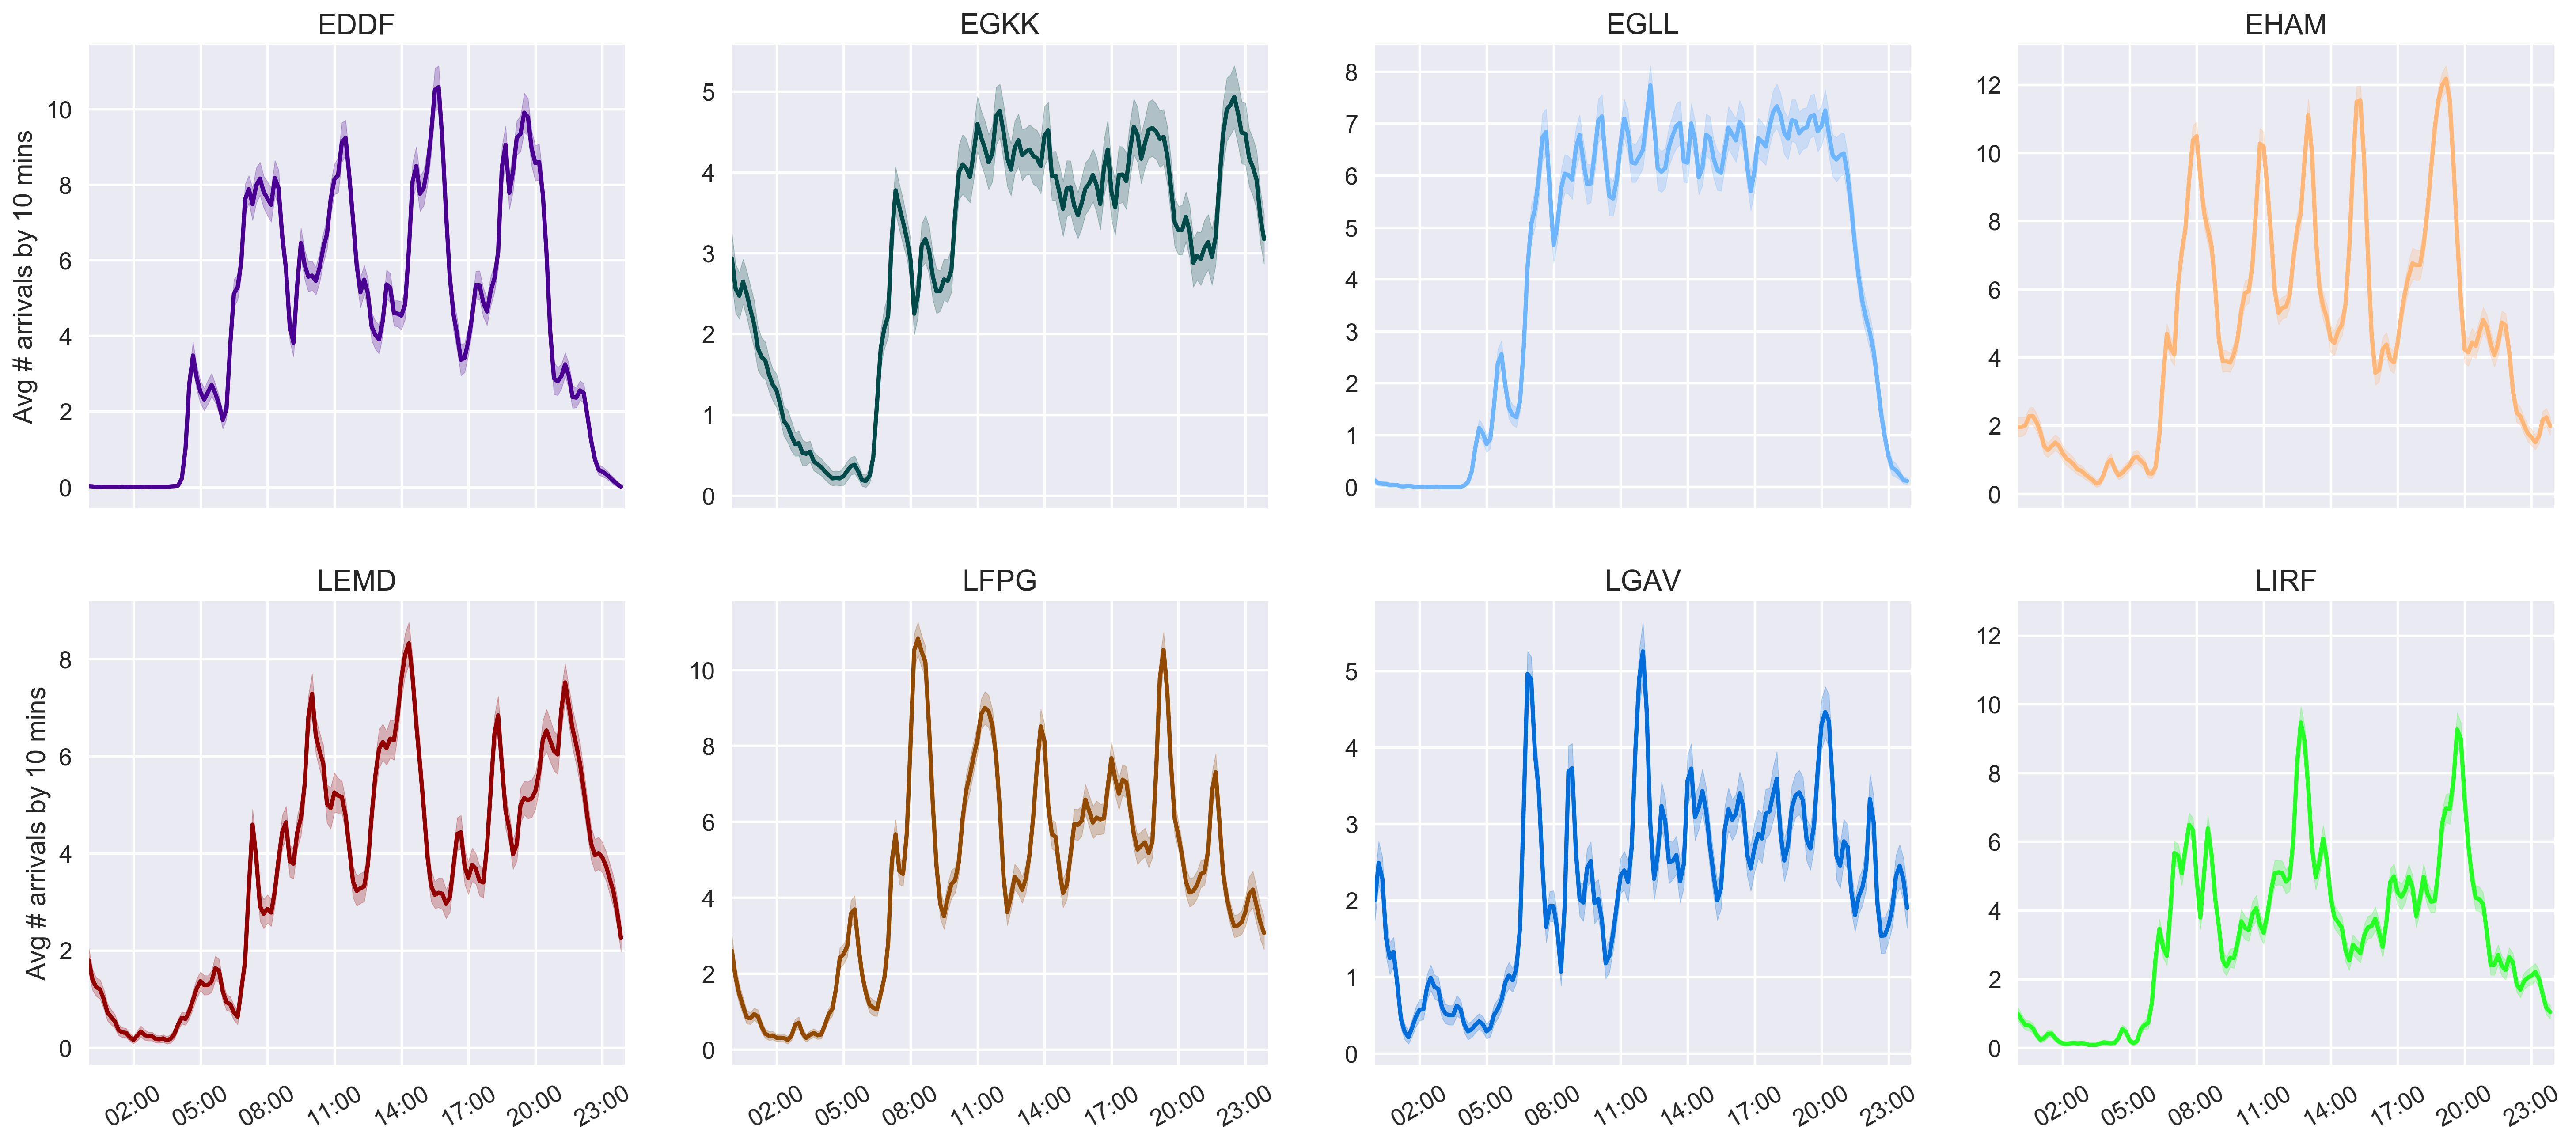
\includegraphics[width=.9\textwidth]{AvgArrivals}
\end{frame}

\begin{frame}[t]\frametitle{Significant autocorrelations at lag 10 mins and 1-2 days}
    \centering
    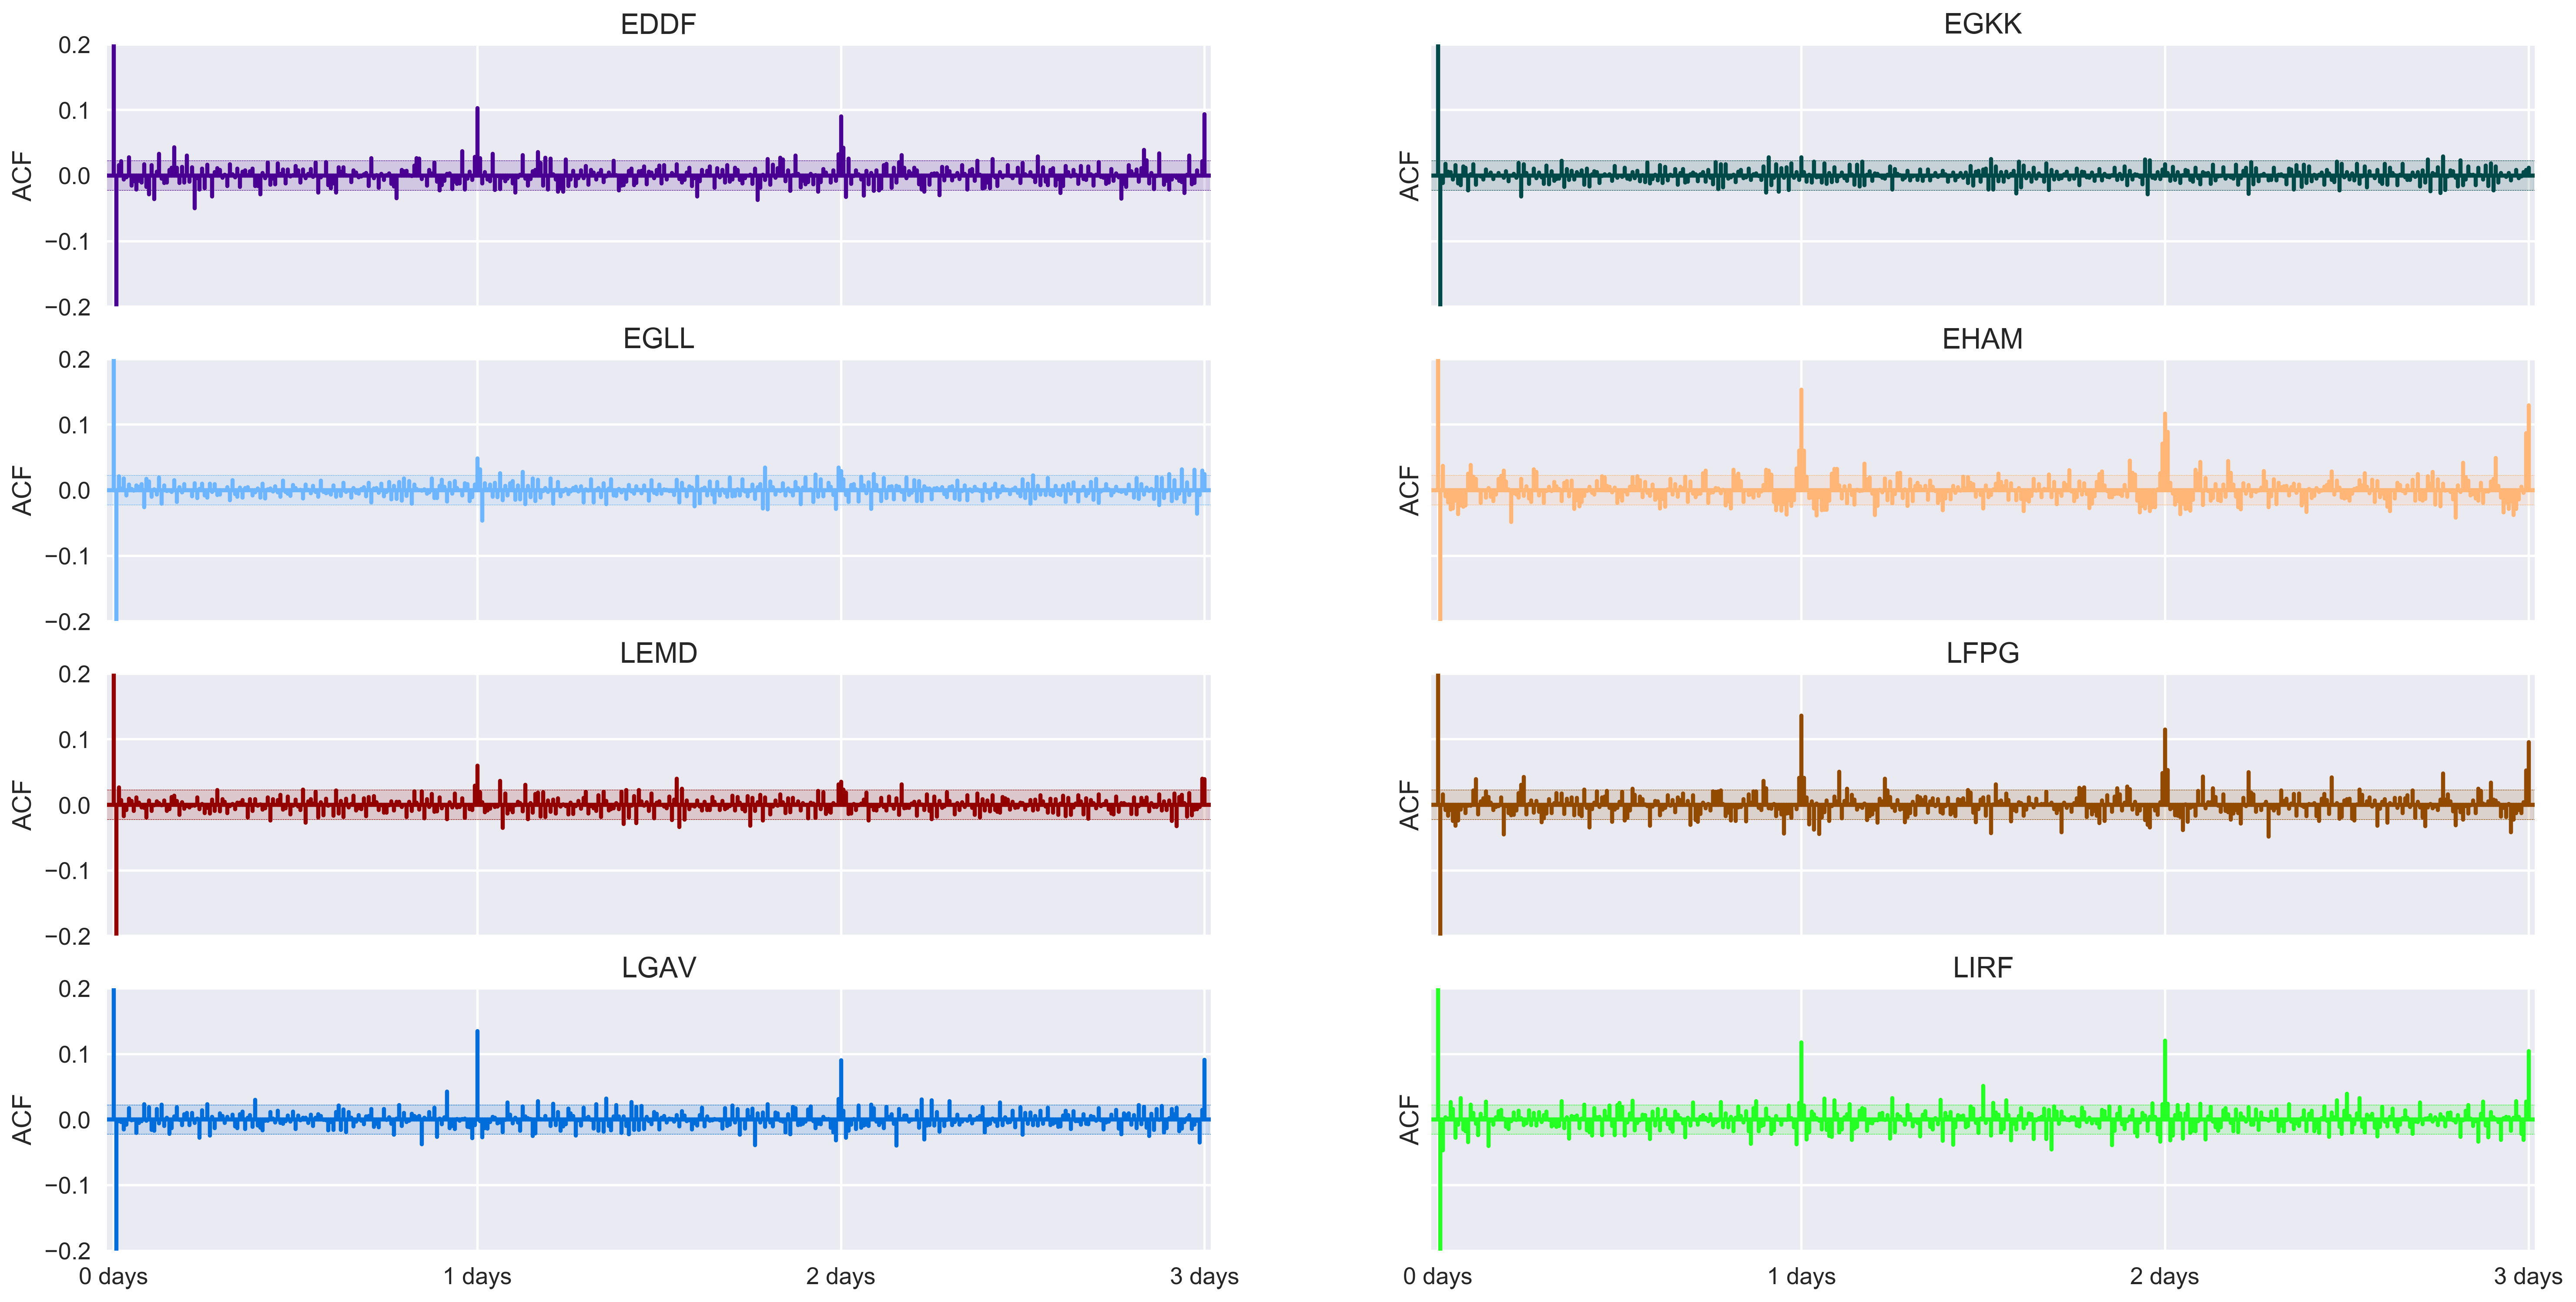
\includegraphics[width=.7\textwidth]{Autocorr}

    \hfill

    We expect \alert{batch arrivals} \emph{(typically Weibull interarrivals)}
    and a \alert{daily-periodic demand}
\end{frame}

\begin{frame}[t]\frametitle{Interarrival times are (nearly) exponential}
    \centering
    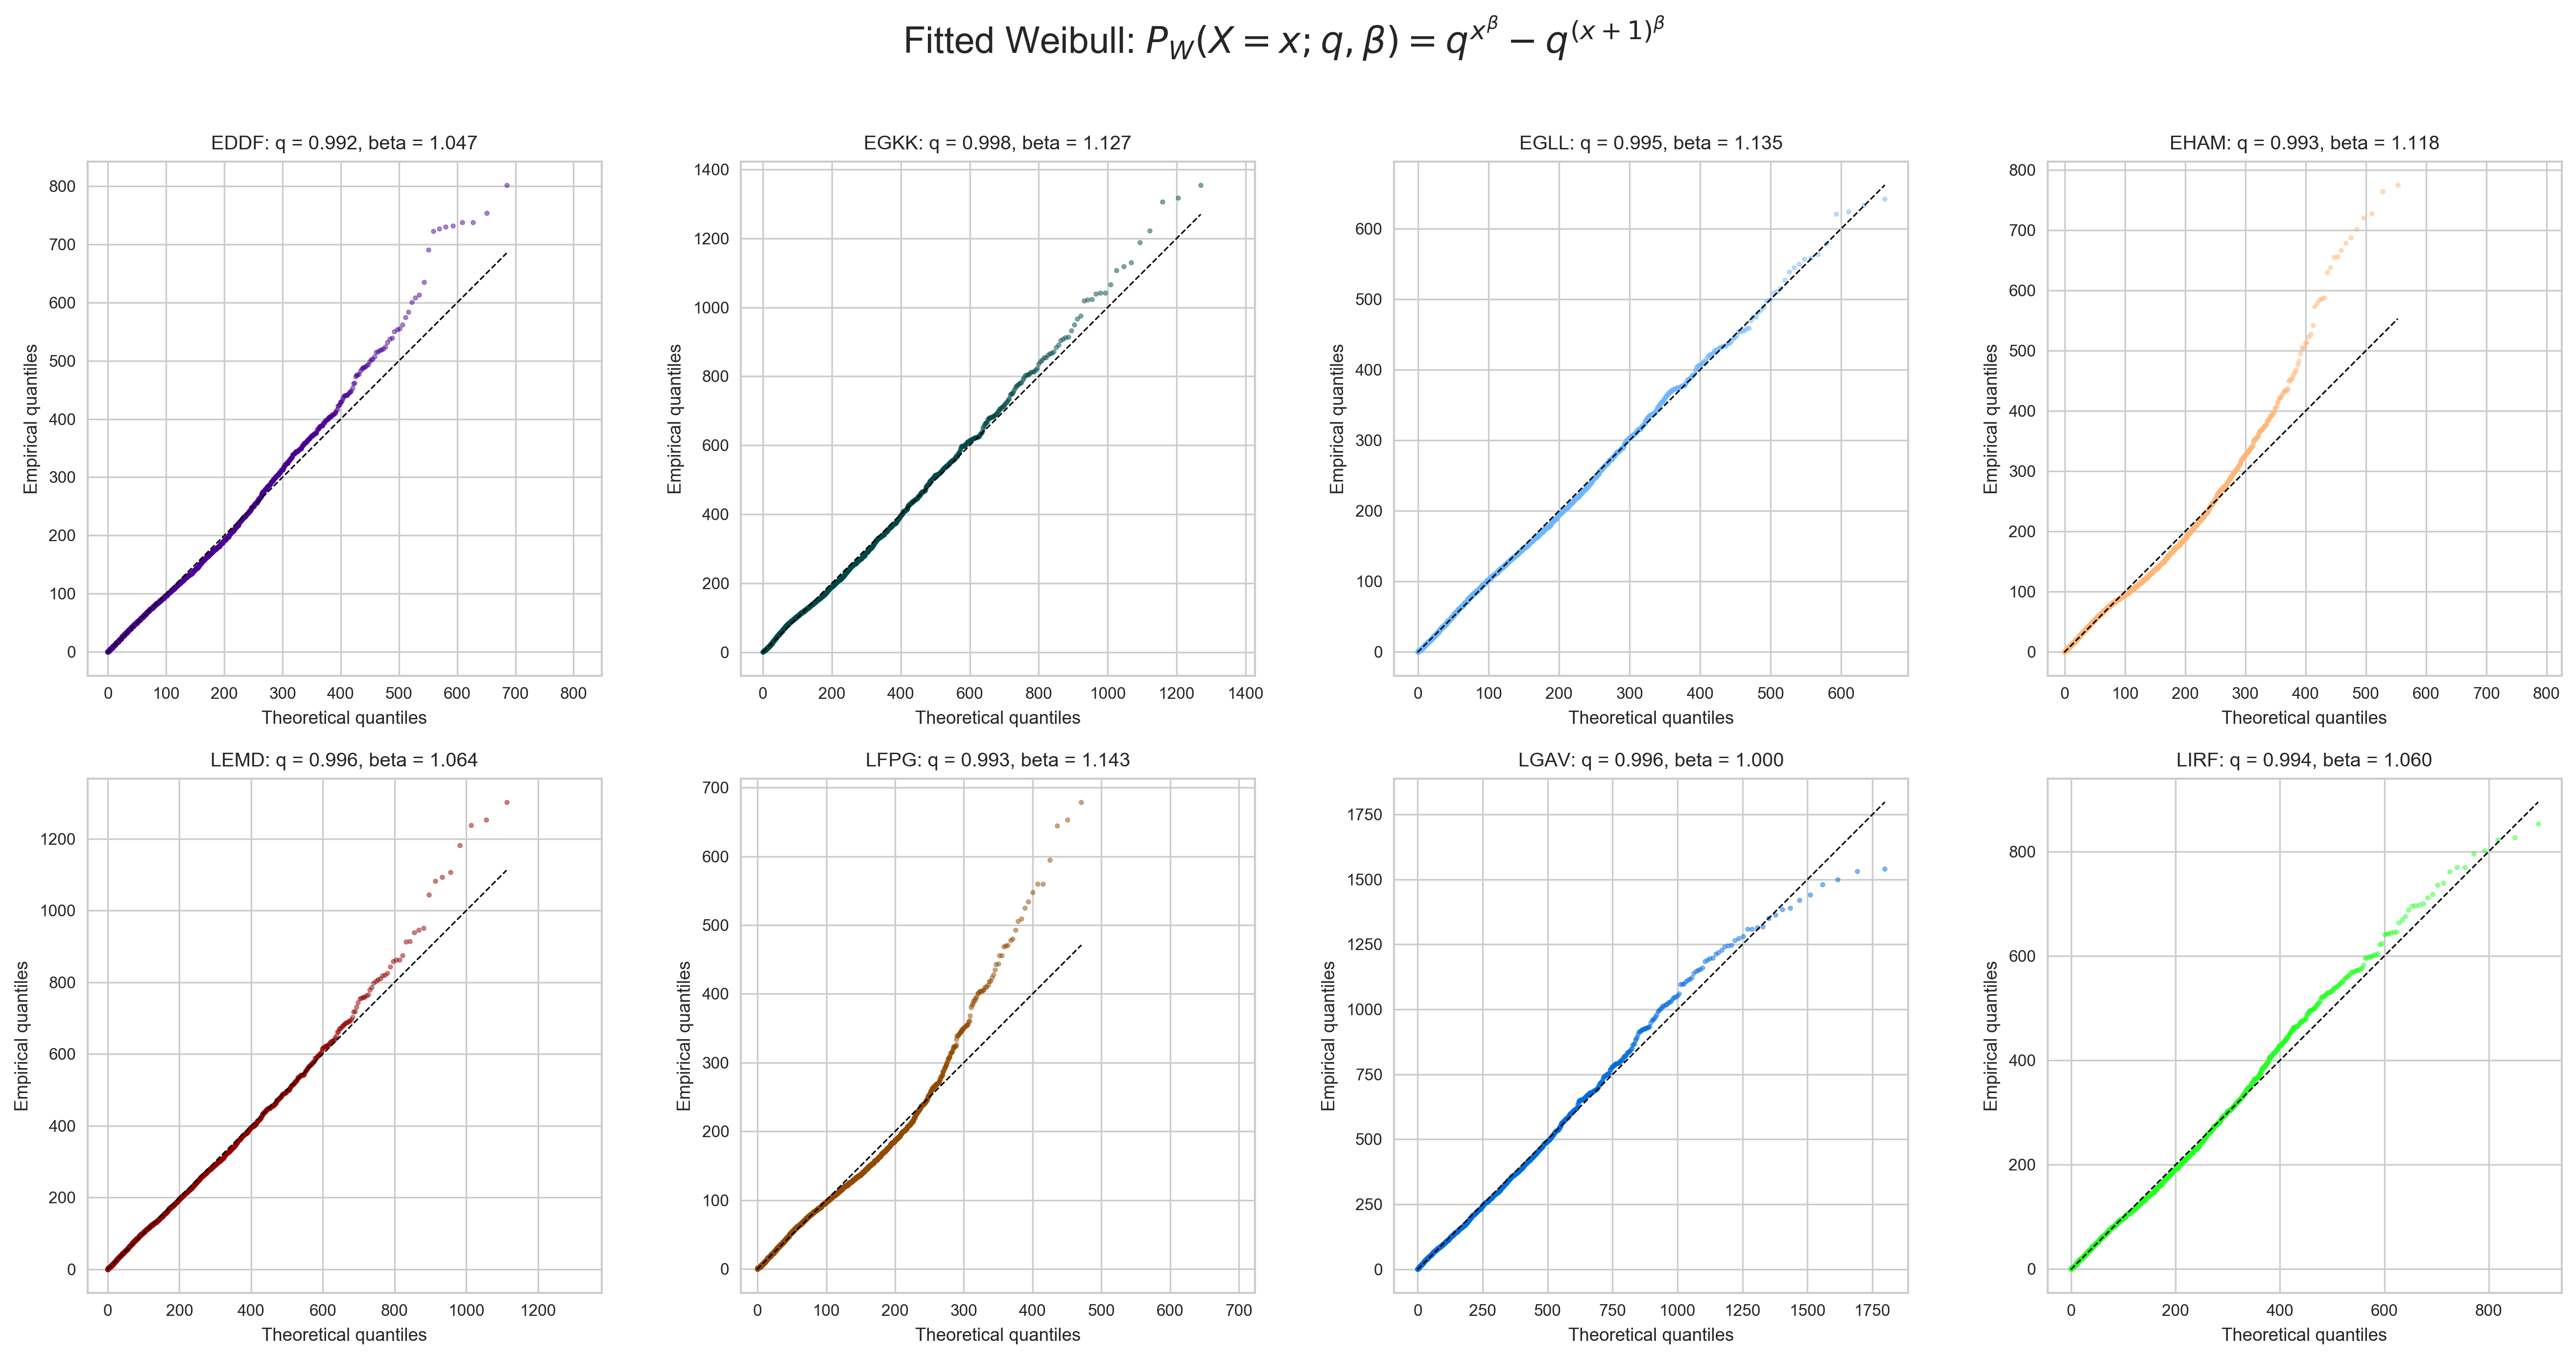
\includegraphics[width=.65\textwidth]{IA_qqplot0800-0930}

    \hfill

    \emph{Poisson process explains shape $\simeq 1.0$
    but clashes with negative lag-1 autocorrelation}
\end{frame}

\begin{frame}[t]\frametitle{Data-driven Poisson process}
    \begin{enumerate}
        \item Aggregate arrivals TS, e.g.\ by intervals of 10 minutes
        \item Run a \alert{changepoint-detection} algorithm, e.g.\ PELT, under the null hypothesis of Poissonian arrivals to obtain
        \begin{itemize}
            \item changepoint time $\hat{t}_k$
            \item $\hat{\lambda}_k$, estimated intensity in $[\hat{t}_k, \hat{t}_{k+1})$
        \end{itemize}
        \item \alert{Cluster} couples $\{(\hat{t}_k, \hat{\lambda}_k)\}_k$, e.g.\ via DBSCAN
        \item Compute the \alert{centroid} $(\bar{t}_i, \bar{\lambda}_i)$ of each cluster
        \item Define a \alert{step-wise, periodic intensity function} that takes on $\bar{\lambda}_i$ for $t \,\in\, [\bar{t}_i, \bar{t}_{i+1})$
    \end{enumerate}
\end{frame}
%
% \begin{frame}[t]\frametitle{Changepoint detection via PELT}
%     \begin{columns}
%         \column{.5\textwidth}
%         \begin{itemize}
%             \item PELT is an algorithm for multiple changepoint detection in a time series
%             \item It can detect changes in mean, variance, or both
%             \item Software available via R package \texttt{changepoint}
%             \item We work under the null hypothesis of Poisson arrivals
%         \end{itemize}
%
%         \column{.5\textwidth}
%         \centering
%         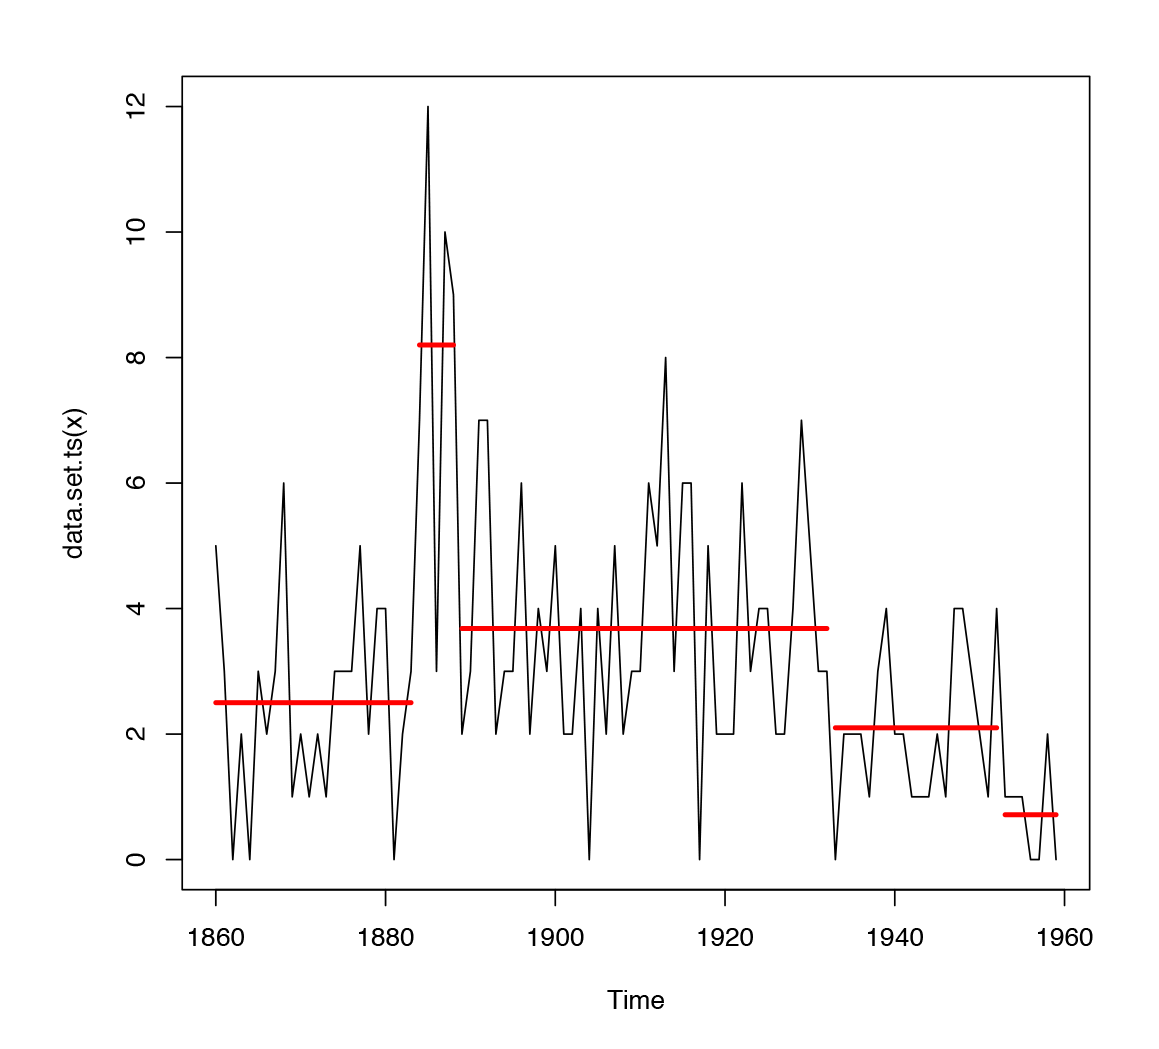
\includegraphics[width=.85\textwidth]{pelt}
%
%         {\tiny Killick, Eckley (2014) \emph{J Stat Soft} 58(3)}
%     \end{columns}
% \end{frame}
%
% \begin{frame}[t]\frametitle{Result of PELT}
%     \centering
%     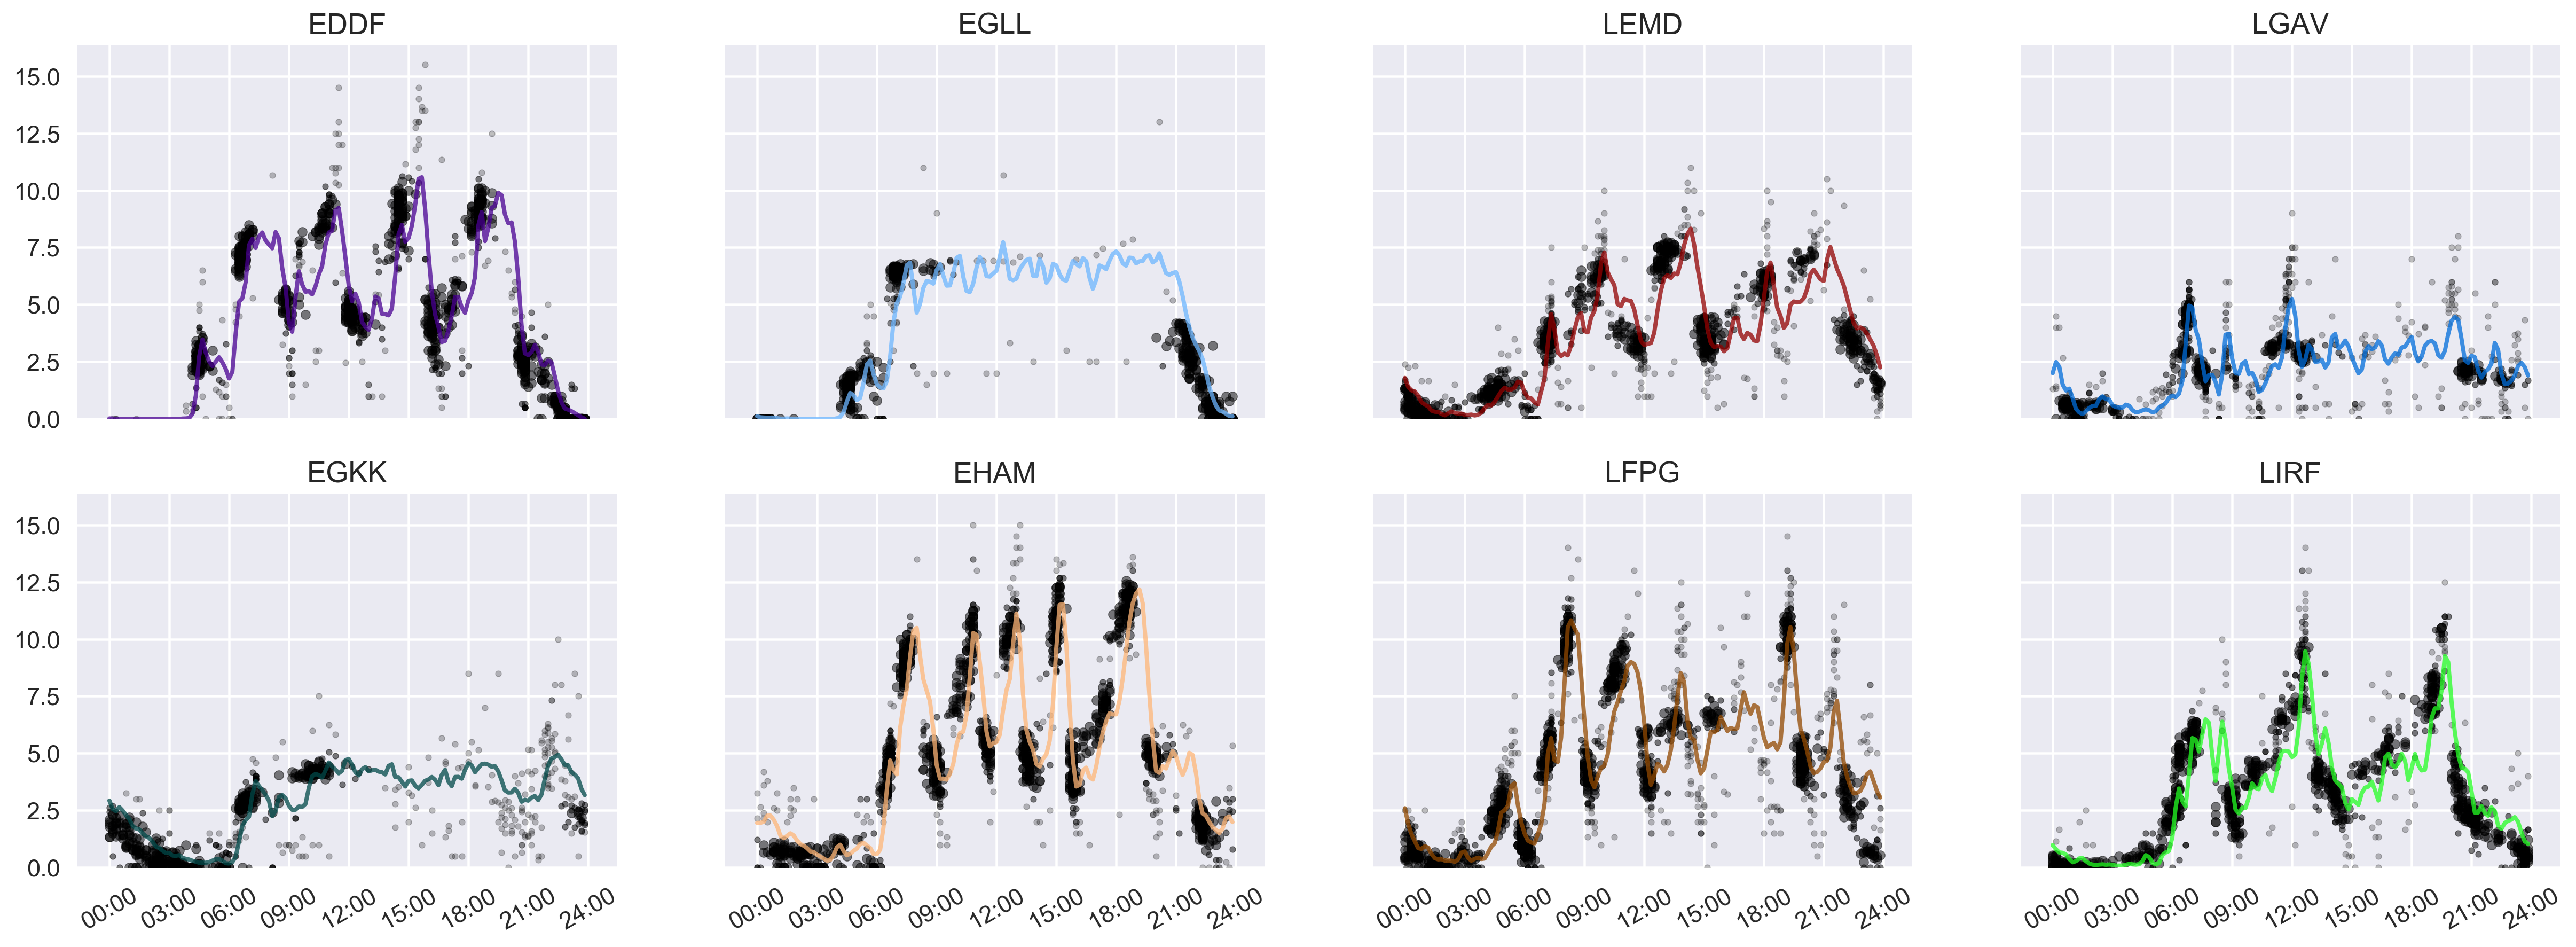
\includegraphics[width=\textwidth]{DDPoisson_precluster}
% \end{frame}
%
% \begin{frame}[t]\frametitle{Clustering via DBSCAN}
%     \begin{columns}
%         \column{.5\textwidth}
%         \begin{itemize}
%             \item Density-based spatial clustering of applications with noise (DBSCAN)
%             \item Two hyperparameters, $\varepsilon$ and $n_{\mathrm{pts}}$
%             \item Core points (red) have at least $n_{\mathrm{pts}}$ other points within distance $\varepsilon$
%             \item Non-core (yellow) lie within $\varepsilon$ from a core point
%             \item The remainders are outliers (blue)
%         \end{itemize}
%
%         \column{.5\textwidth}
%         \centering
%         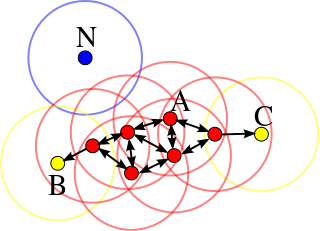
\includegraphics[width=.85\textwidth]{dbscan}
%
%         {\tiny Source: Wikimedia Commons}
%     \end{columns}
% \end{frame}
%
\begin{frame}[t]\frametitle{Implementation of data-driven Poisson process}
    \centering
    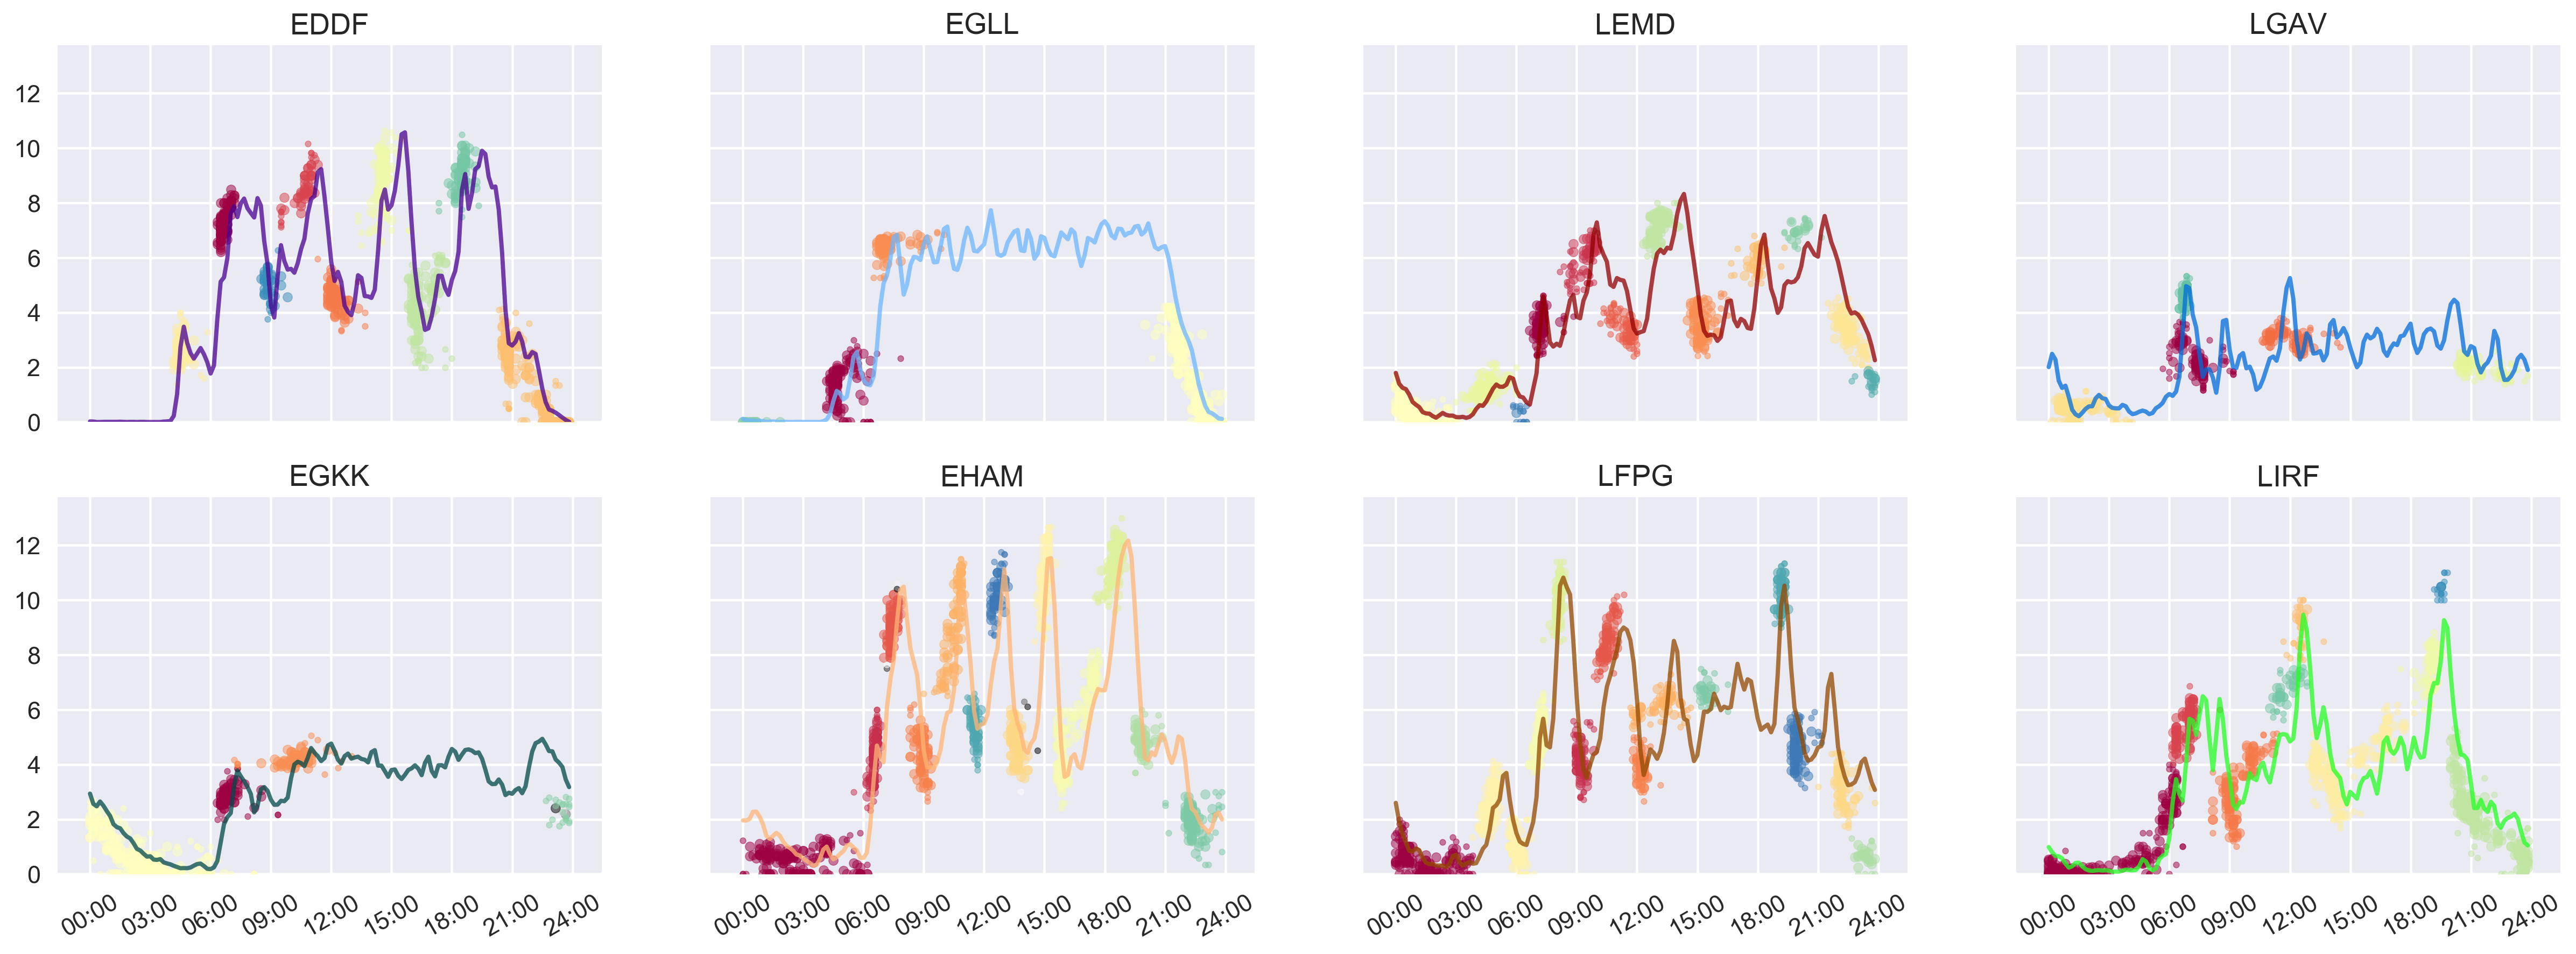
\includegraphics[width=\textwidth]{DDPoisson}
\end{frame}

% \begin{frame}[t]\frametitle{Pre-scheduled random arrivals (PSRA)}
%     \centering
%     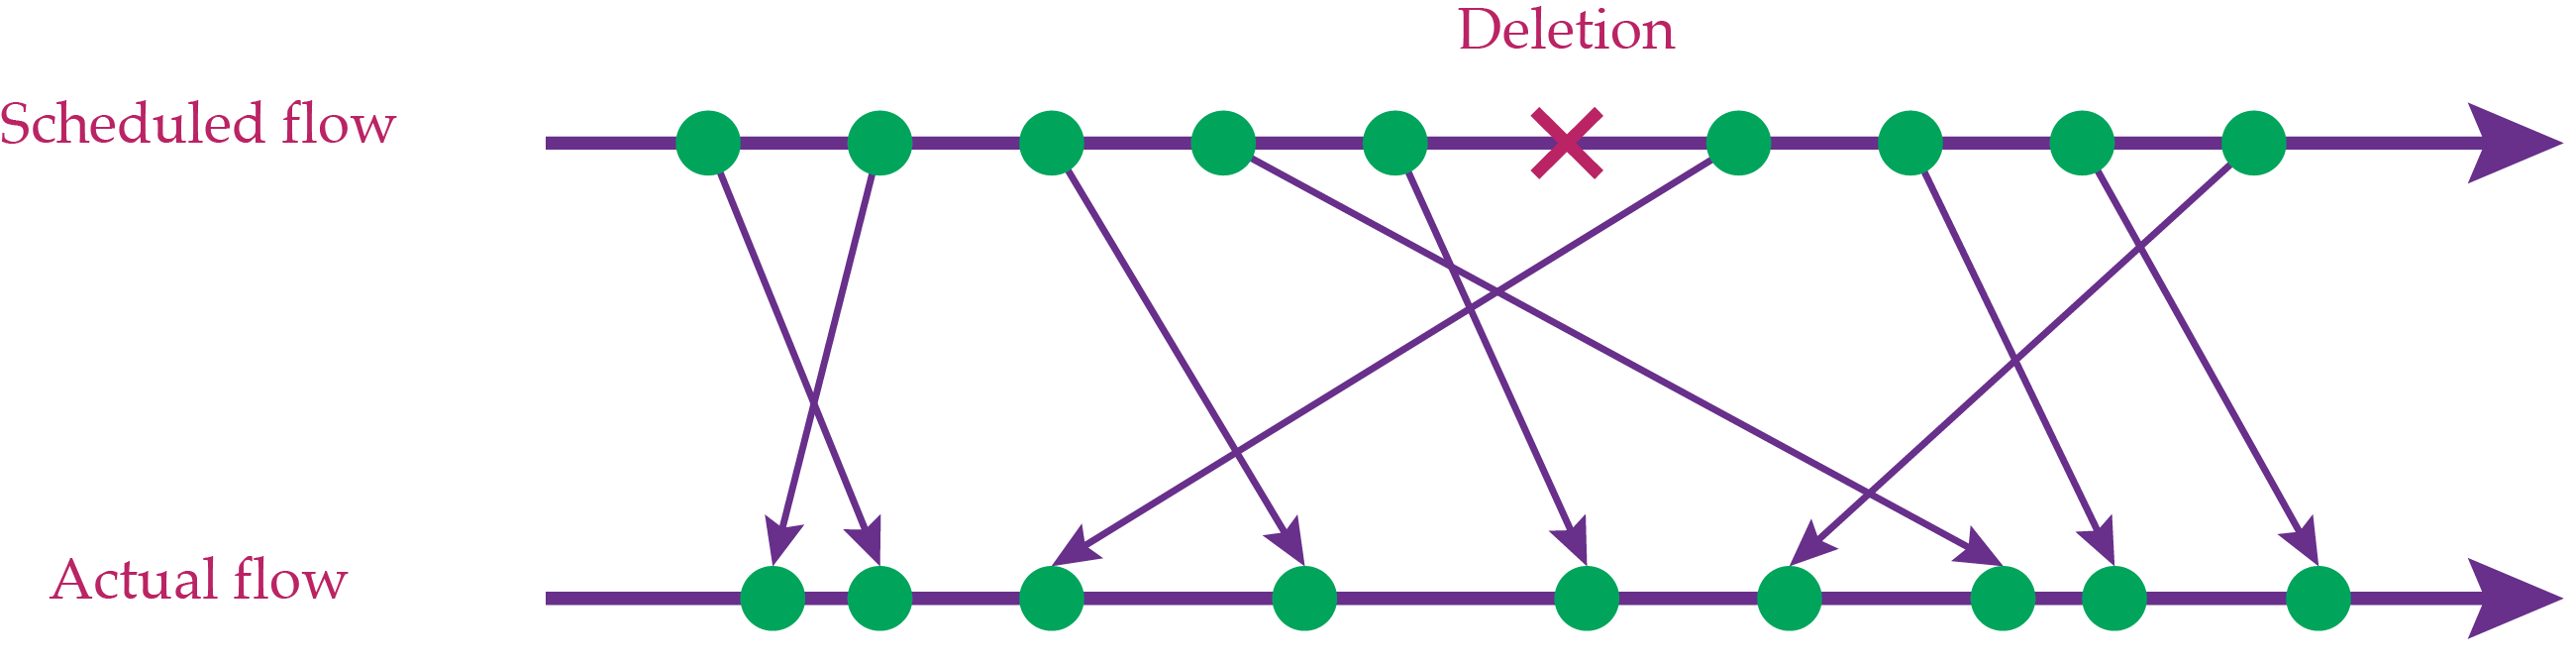
\includegraphics[width=.65\textwidth]{psra-1}
%
%     {\tiny From Caccavale et al. (2014) \emph{J Air Transp Manag}, 34, 116--122}
%
%     \vfill
%
%     \begin{alertblock}{Idea}
%         Fixed, deterministic schedule perturbed by IID random variables
%         \[ t_i = \frac{i}{\mu} + \xi_i \]
%         \emph{\alert{Note.} It weakly converges to Poisson process
%         when delays's standard deviation $\sigma_{\xi} \to \infty$}
%     \end{alertblock}
% \end{frame}

\begin{frame}[t]\frametitle{Data-driven PSRA}
    \begin{alertblock}{Recall}
        Fixed, deterministic schedule perturbed by i.i.d.\ random variables
        \[ t_i = \frac{i}{\lambda} + \xi_i \]
    \end{alertblock}
    \begin{enumerate}
        \item Let $t^{\mathrm{M3}}_i$ the \alert{\emph{actual} arrival} time at 40 NM
        \item Let $t^{\mathrm{M1}}_i$ the \alert{\emph{anticipated} arrival} time at 40 NM (from the last flight plan agreed with Eurocontrol)
        \item Compute the \emph{delays} $\delta_i = t^{\mathrm{M3}}_i - t^{\mathrm{M1}}_i$
        \item Define
        \[t_i = t^{\mathrm{M1}}_i + \xi_i\]
        where $\{\xi_i\}_i$ are IID rvs drawn from the empirical distribution of the delays $\{\delta_i\}_i$
    \end{enumerate}
\end{frame}

\begin{frame}[t]\frametitle{Data-driven Poisson vs PSRA}
    \centering
    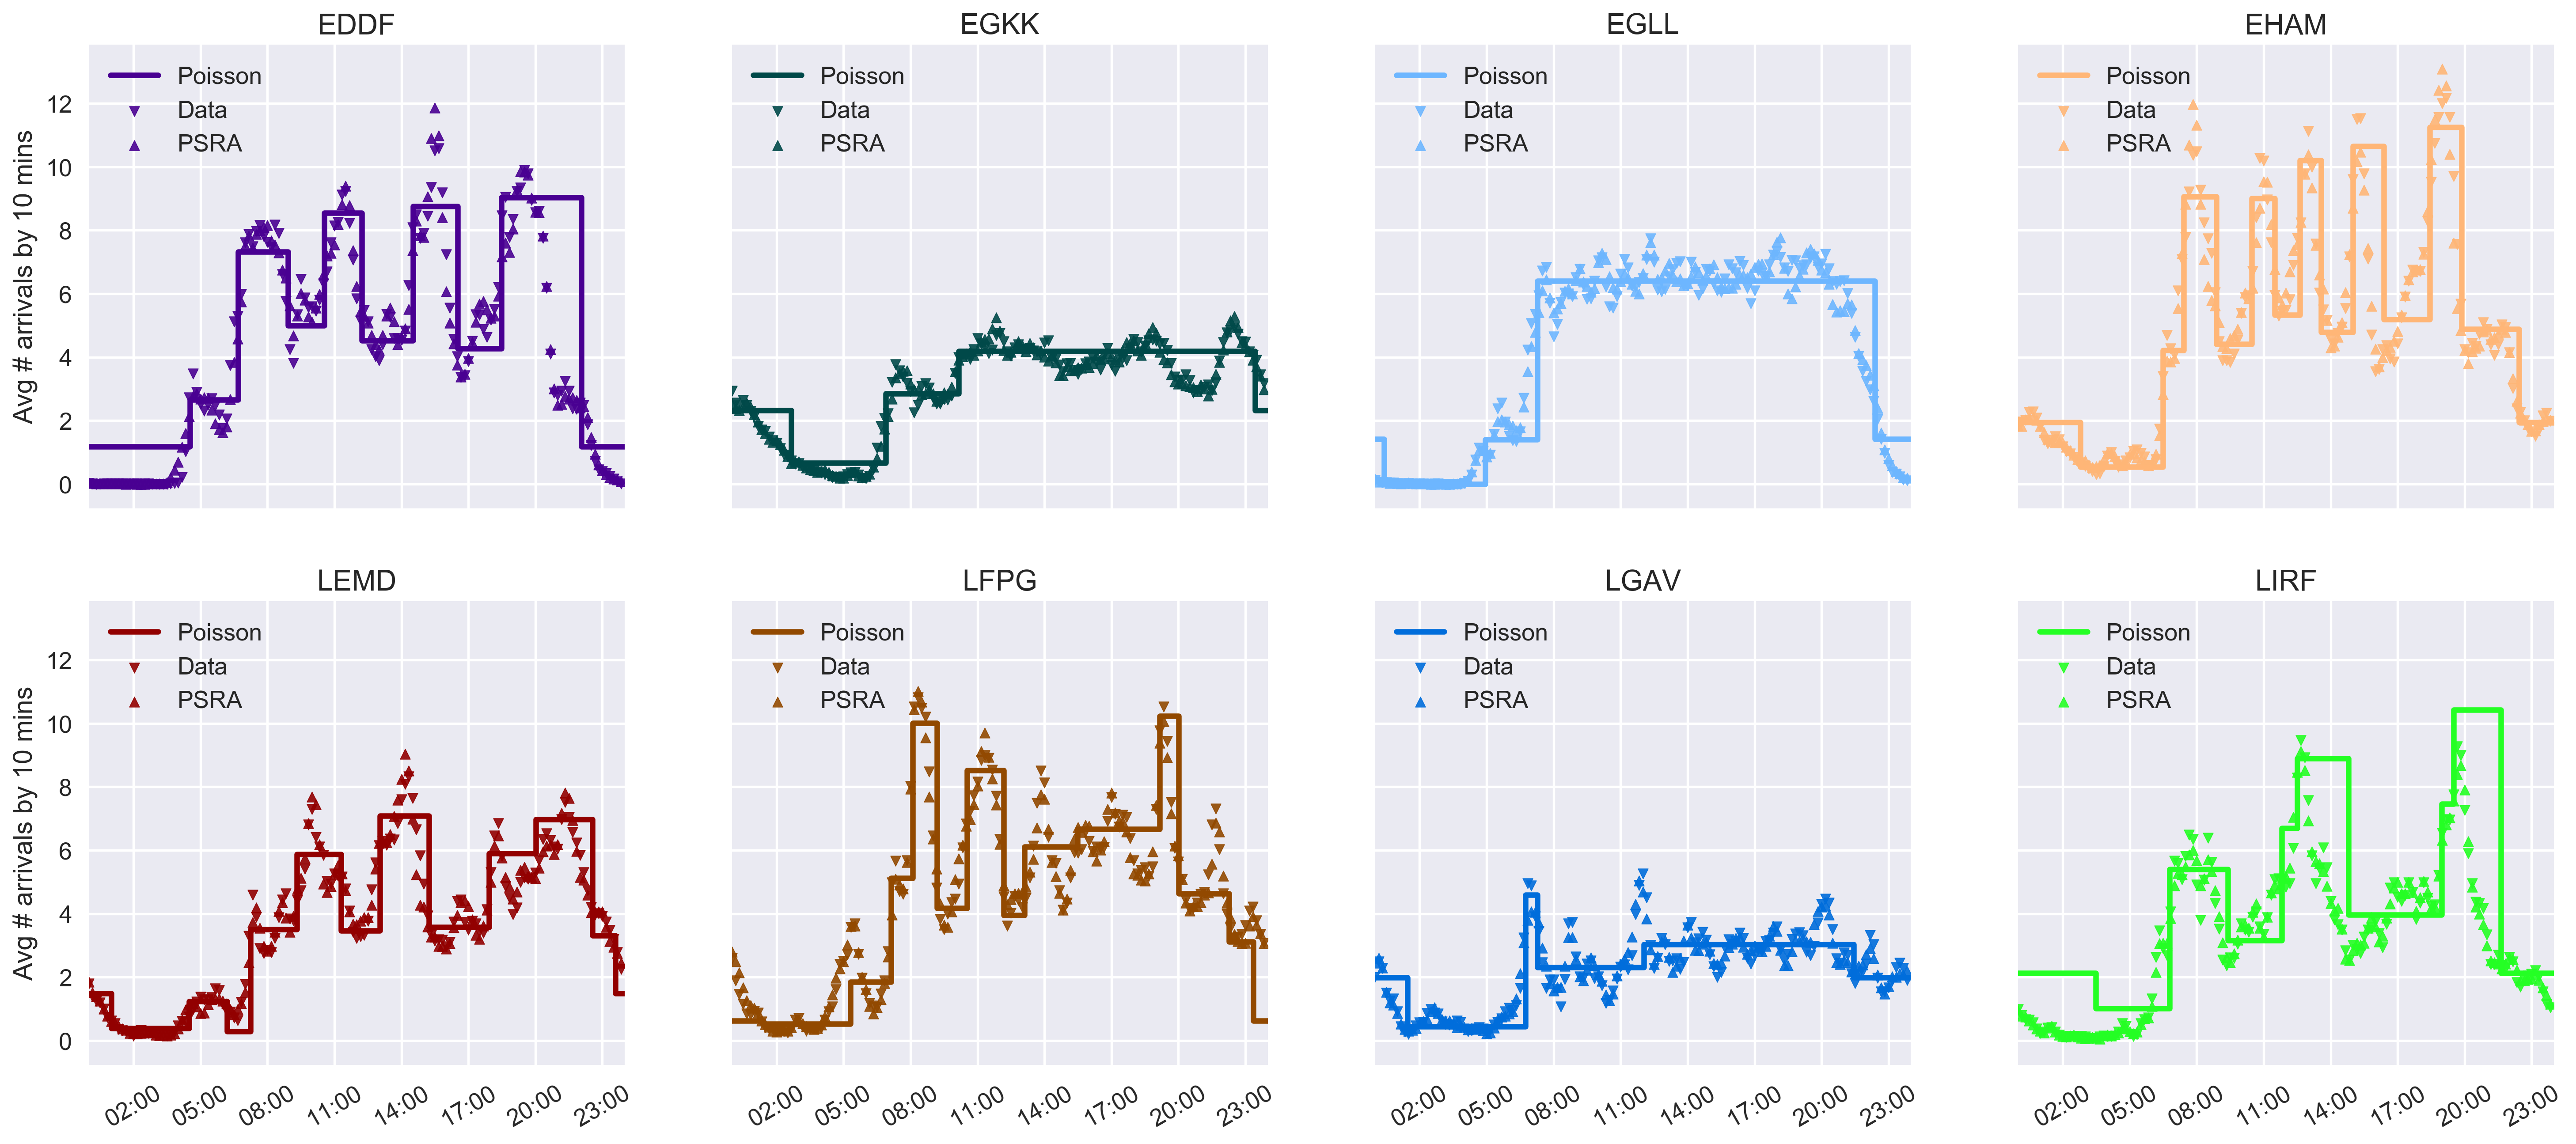
\includegraphics[width=.9\textwidth]{mean_simul_arrivals}
\end{frame}

\begin{frame}[t]\frametitle{Data-driven Poisson vs PSRA}
    \begin{itemize}
        \item PSRA outperform Poisson arrivals in reproducing the average daily demand
        \item Average demand reproduced with Poisson model by \alert{forcing}
        intensity to vary over a finer time scale, e.g.\ every 10 minutes
        \begin{itemize}
            \item \alert{\textsc{Caveat}} number of parameters required increases in a sensible manner (144)
            \item \alert{\textsc{Caveat}} system mostly out of equilibrium
            \item \alert{\textsc{Caveat}} mathematical tractability is greatly reduced
        \end{itemize}
        \item PSRA has 1 parameter at most
        \item PSRA inherits \alert{arrivals correlation-structure} from the M1 schedule
        \item In contrast, Poissonian arrivals have \alert{independent increments} by definition
    \end{itemize}
\end{frame}

\begin{frame}[t]\frametitle{Arrivals correlation}
    \centering
    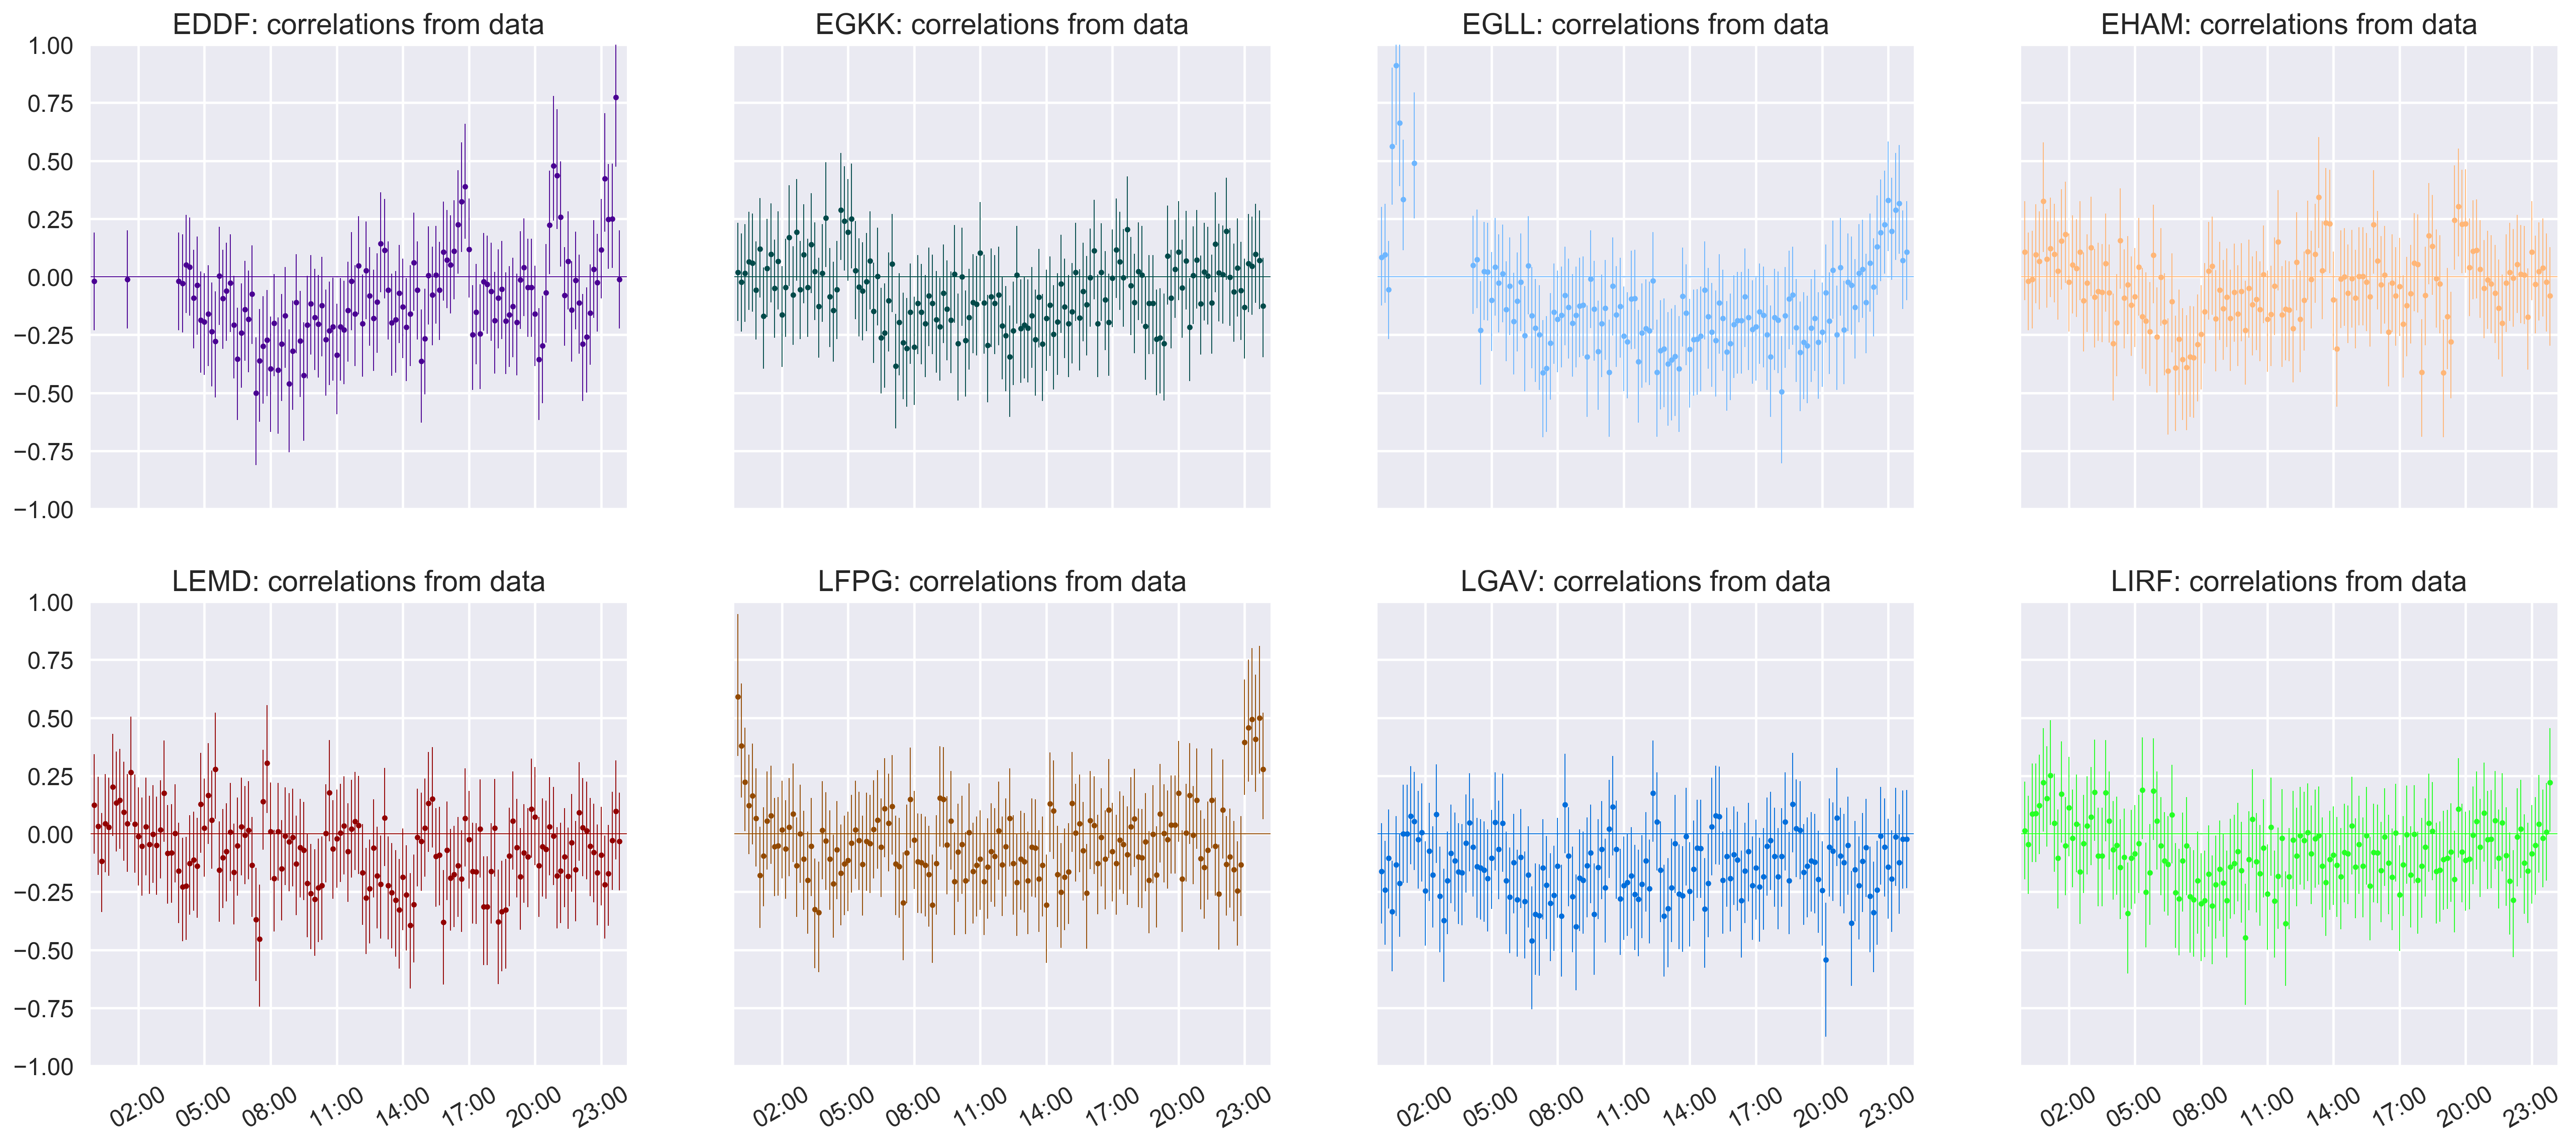
\includegraphics[width=.9\textwidth]{correlations_true}
\end{frame}

\begin{frame}[t]\frametitle{Correlations from simulation of PSRA}
    \centering
    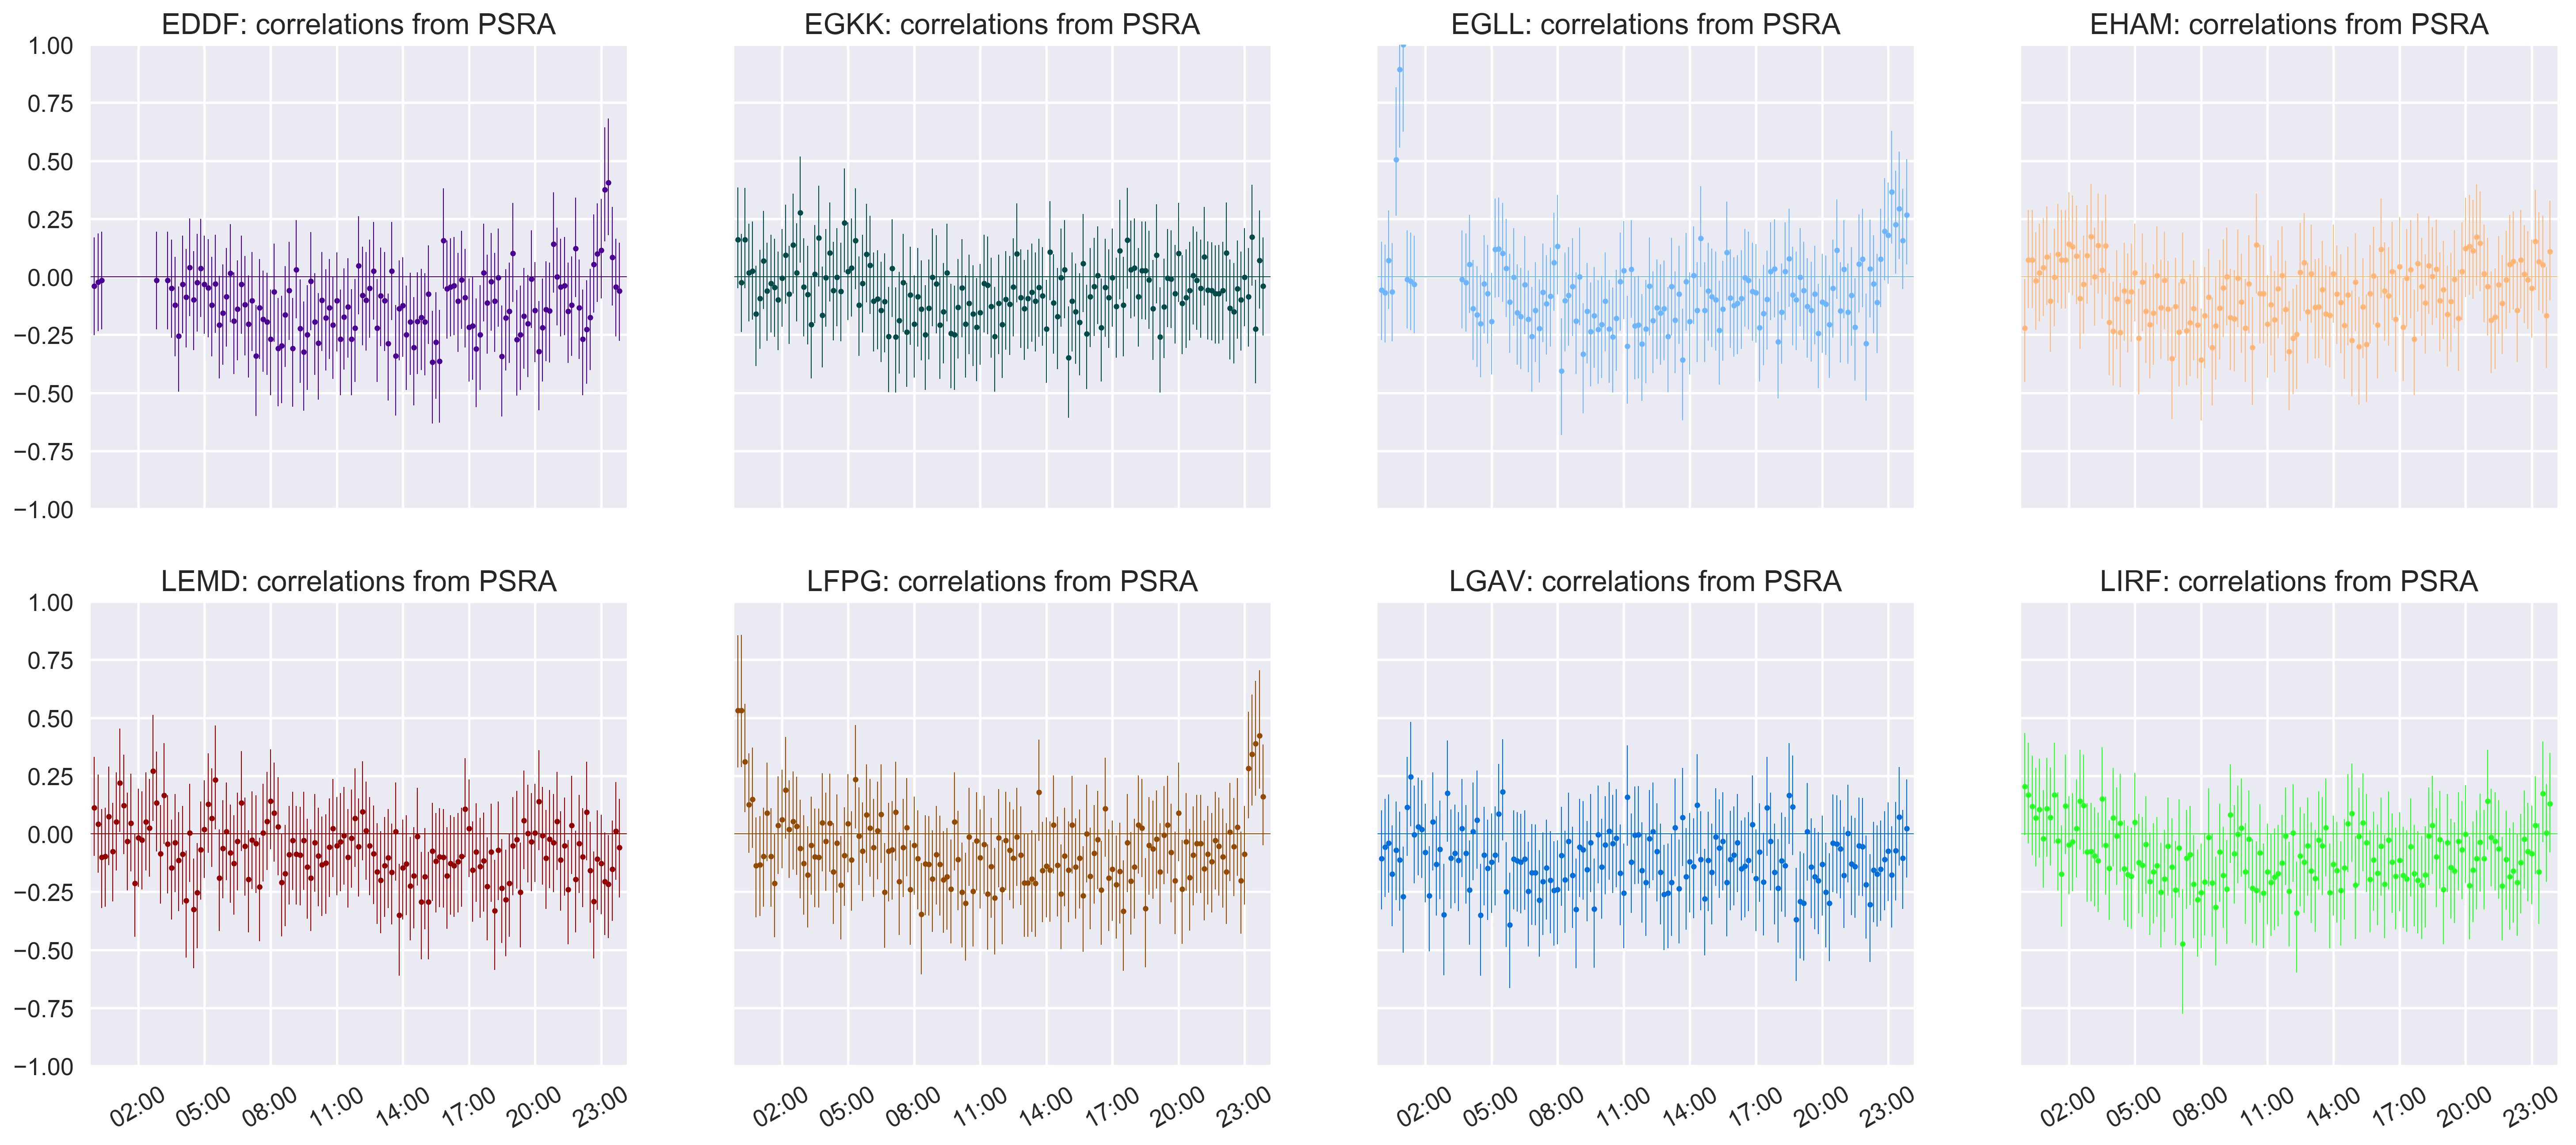
\includegraphics[width=.9\textwidth]{correlations_psra}
\end{frame}

\section{Exponentially Delayed Arrivals}

\begin{frame}[t]\frametitle{The EDA/D/1 queue model}
    \begin{block}{Exponentially Delayed Arrivals (EDA)}
        Particular case of PSRA ($\lambda = 1$ for convenience)
        \[t_i = i + \xi_i\,,\]
        where now $\xi_i$ are independent exponential random variables, i.e.\
        \[f_\xi(t) =
        \begin{cases}
            \beta\,e^{-\beta\,t} \qquad & \text{if } t>0\,,\\
            0 & \text{otherwise.}
        \end{cases}
        \]
    \end{block}
    \begin{block}{Thinning}
        Each customer is deleted independently with probability
        $1-\rho$, whereas it is kept with probability $\rho$.
    \end{block}
\end{frame}

\begin{frame}[t]\frametitle{The EDA/D/1 queue model}
    \begin{block}{Probability of a customer arriving/not arriving in each slot}
        \[p = \int_0^1 f_\xi(t)\, dt = 1-e^{-\beta} \quad,\quad q=1-p=e^{-\beta}\]
    \end{block}
    \begin{center}
        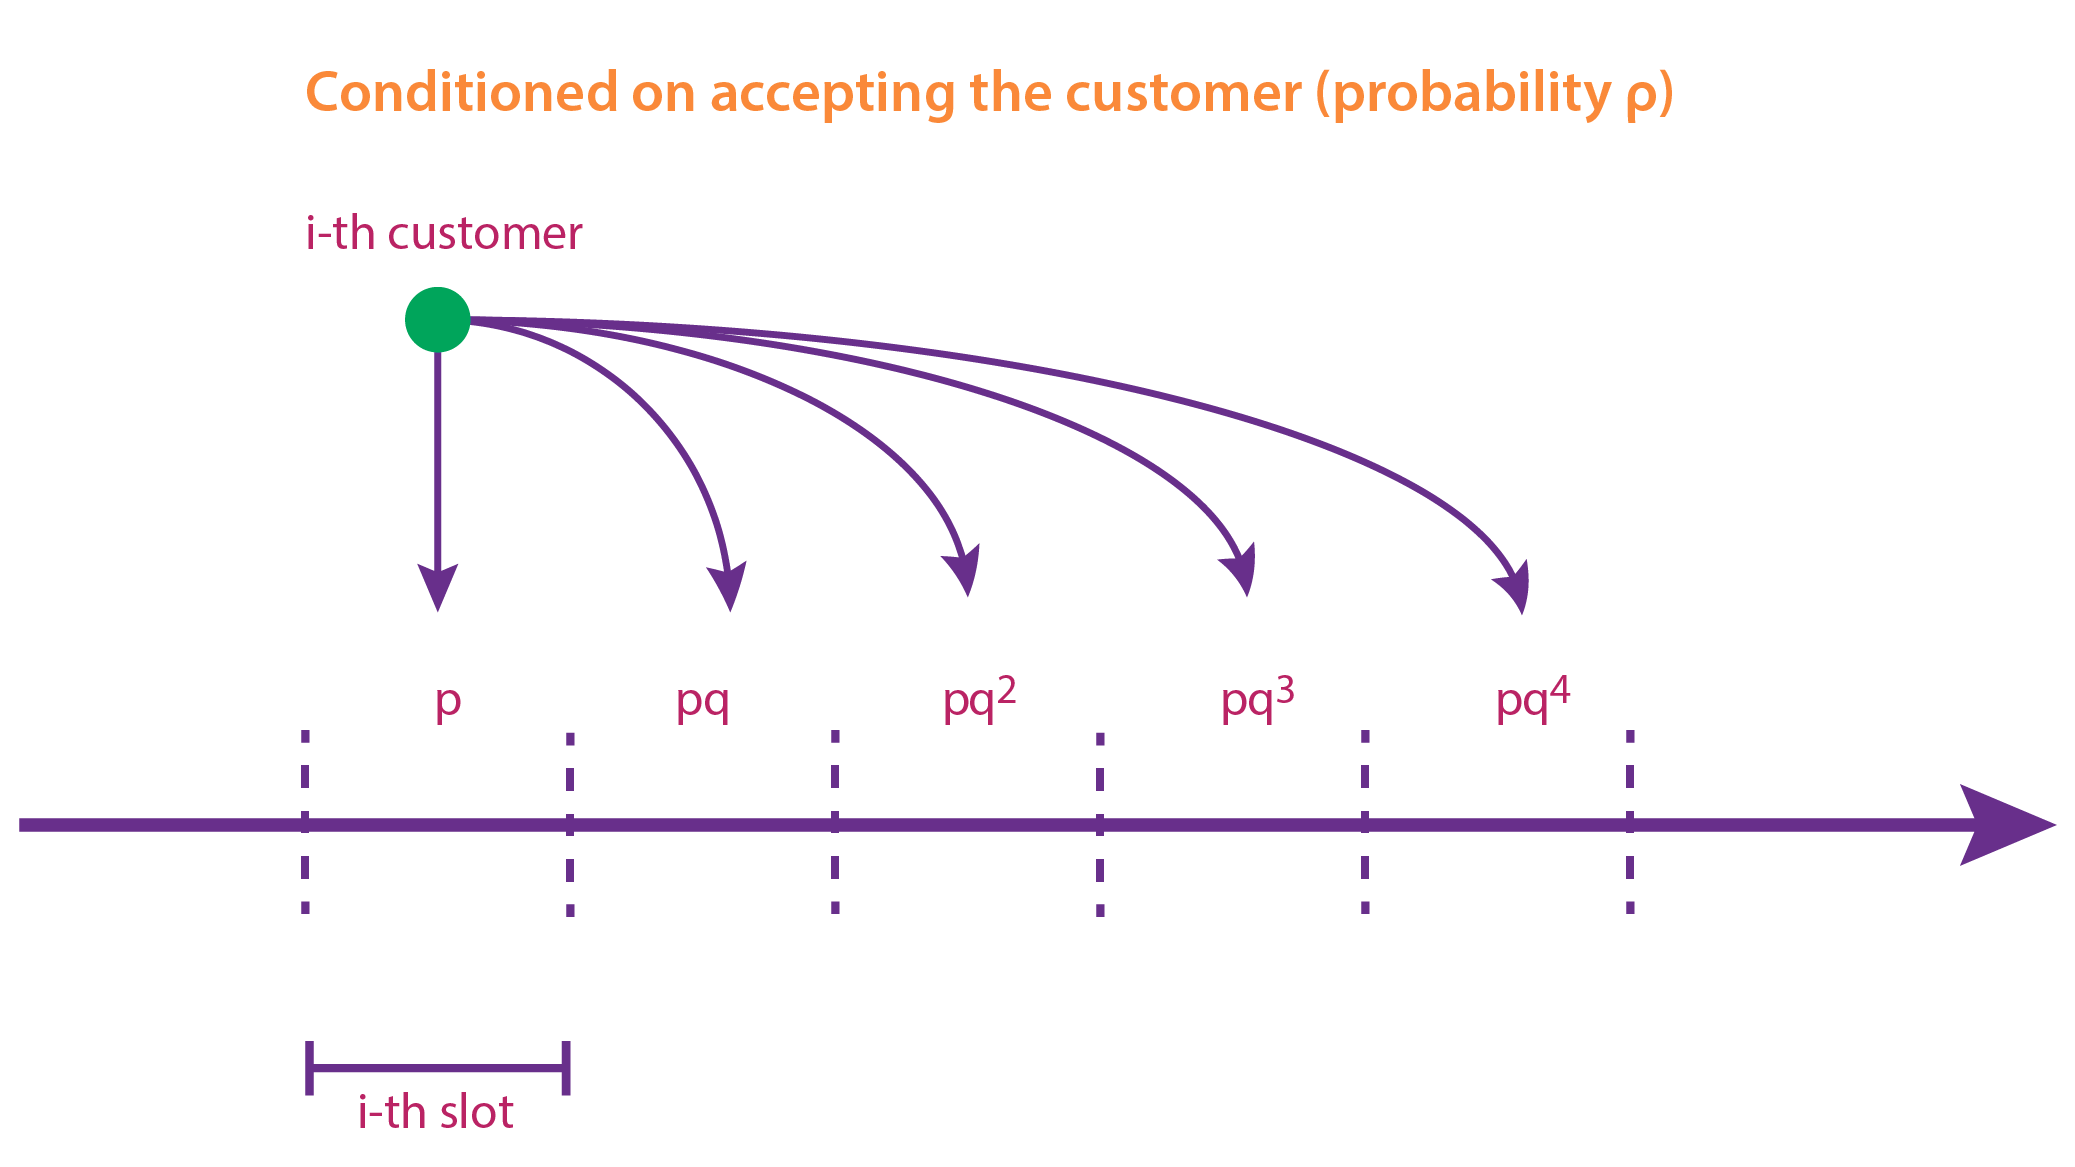
\includegraphics[width=0.7\textwidth]{eda}
    \end{center}
\end{frame}

\begin{frame}[t]\frametitle{The EDA/D/1 queue model}
    \begin{exampleblock}{Previous results about EDA}
        \begin{itemize}
            \item \emph{Winstein, 1959.} Solution for general delays $\xi_i \in [0,2]$ and exponential service times;
            \item \emph{Mercer, 1960.} Continuation of Winsten's studies;
            \item \emph{Lewis, 1961.} Statistical properties of inter-arrivals;
            \item \emph{Kendall, 1964.} Arrival process seen as output of stationary $D/M/\infty$ system;
            \item \emph{Nelsen and Williams, 1970.} Exact characterization for the distribution of
            the inter-arrival time intervals;
            \item After that, only numerical studies applied to trasportation systems, outpatient scheduling and crane handling optimization.
        \end{itemize}
    \end{exampleblock}
\end{frame}

\begin{frame}[t]\frametitle{System recursion}
    \begin{block}{Queue length at time $t$}
        \[n_{t+1}= n_t + a_{(t,t+1]} -(1-\delta_{n_t,0})\]
        where $a_{(t,t+1]}$ is the number of arrivals in the interval $(t,t+1]$.
        \begin{center}
            \alert{This quantity does depend on the whole trajectory up to
            time $t$!}
        \end{center}
    \end{block}
    \begin{block}{How many arrivals in the unit interval?}
        In the interval $(t,t+1]$ there may arrive
        \begin{itemize}
            \item the t-th customer, provided it is not deleted;
            \item any of the $l_t$ customers that have not been deleted and have
            not yet arrived at time $t$.
        \end{itemize}
    \end{block}
\end{frame}

\begin{frame}[t]\frametitle{System recursion}
    \begin{block}{Queue length at time $t$}
        \[n_{t+1}= n_t + a_{(t,t+1]} -(1-\delta_{n_t,0})\]
        where $a_{(t,t+1]}$ is the number of arrivals in the interval $(t,t+1]$.
        \begin{center}
            \alert{This quantity does depend on the whole trajectory up to
            time $t$!}
        \end{center}
    \end{block}
    \vfill
    \begin{alertblock}{Number of arrivals in a slot}
        \[
        \mathbb{P}\left(a_{(t,t+1]}=j \;\Big\vert\; l_t=k \right) =
        \begin{cases}
            {k\choose j} p^j \, q^{k-j} \qquad &\text{deletion at time $t$}\\
            {k+1\choose j} p^j \, q^{k+1-j} \qquad &\text{otherwise}
        \end{cases}
        \]
    \end{alertblock}
\end{frame}

\begin{frame}[t]\frametitle{EDA/D/1 as a random walk in the quarter plane}
    \begin{columns}
        \column{0.63\textwidth}
        \centering
        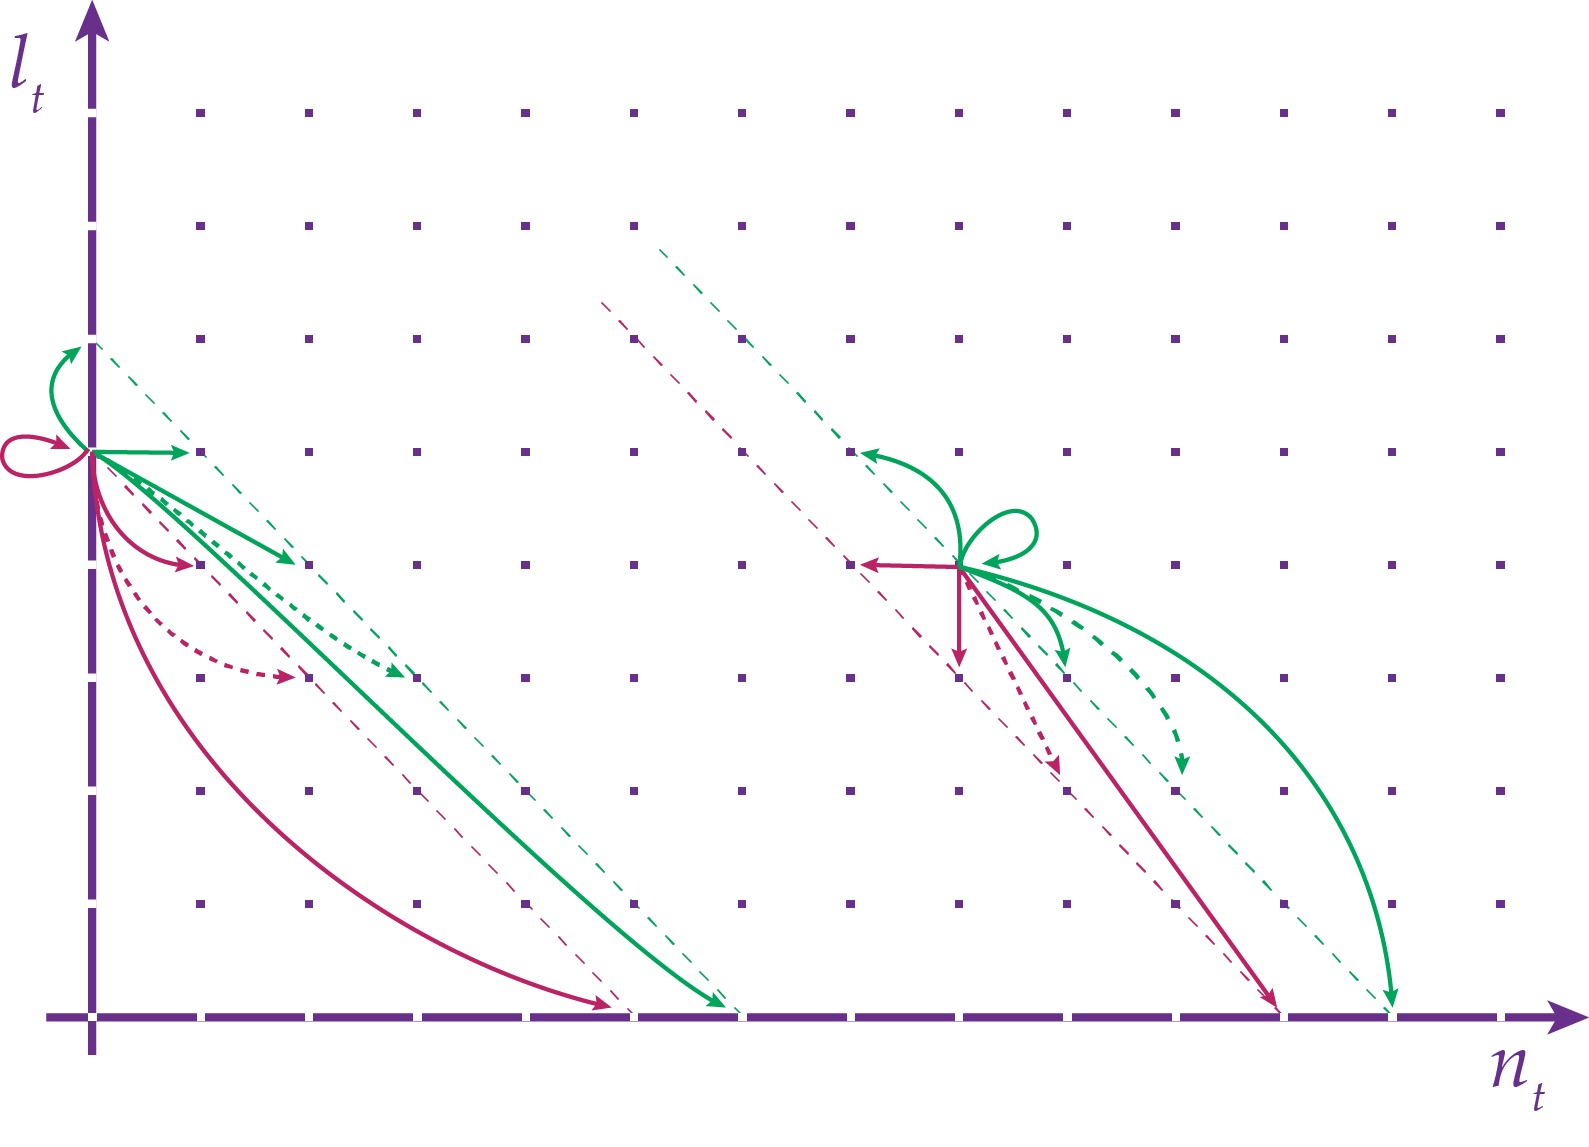
\includegraphics[width=\textwidth]{quarterplane}
        \column{0.35\textwidth}
        \begin{itemize}
            \item $l_t$, number of late customers at time $t$
            \item $n_t$ depends only on $n_{t-1}$ and $l_{t-1}$
            \item $(n_t, l_t)$ is a bivariate Markov chain
        \end{itemize}
    \end{columns}
\end{frame}

\begin{frame}
    \frametitle{Existence of a unique stationary state}
    \begin{itemize}
        \item $(n_t, l_t)$ is \emph{positive recurrent}, i.e.\ finite
        mean first return time to any state
        \item This is a consequence of the \emph{stochastic stability} of
        the system for $q, \rho < 1$
        \item Use Foster's criterion with the Lyapunov function
        \[V(n_t, l_t) = M\alpha_t + l_t +1\,,\] where
        \begin{itemize}
            \item $M = \nicefrac{2}{1-\rho}$
            \item $\alpha_t = (n_t+l_t)$
        \end{itemize}
    \end{itemize}
\end{frame}

% \begin{frame}[t]\frametitle{Equilibrium equations}
%   Let $P_{n,l}$ be the unique stationary measure of $(n_t, l_t)$. Then,
%   \begin{align*}
%     P_{0,0} &= (1-\rho)(P_{1,0}+P_{0,0}) \\
%     P_{0,l} &= (1-\rho)(P_{1,l}+P_{0,l})q^l + \rho(P_{1,l-1}+P_{0,l-1})q^l\\
%     P_{n,l} &= (1-\rho)\Bigg[ \sum_{j=0}^n P_{j+1, l+n-j} b_{n-j, l+n-j} + P_{0,l+n} b_{n, l+n}\Bigg]\\
%            &+ \rho\Big[ \sum_{j=0}^n P_{j+1, l+n-j-1} b_{n-j, l+n-j} + P_{0,l+n-1} b_{n, l+n}  \Bigg]
%     % P_{n,l} &= (1-\rho)\Bigg[ \sum_{j=0}^n P_{j+1, l+n-j}\binom{l+n-j}{n-j}p^{n-j}q^{l} \\
%     %        & \qquad\qquad\qquad\qquad\qquad + P_{0,l+n}\binom{l+n}{n}p^nq^l  \Bigg]\\
%     %        &+ \rho\Big[ \sum_{j=0}^n P_{j+1, l+n-j-1}\binom{l+n-j}{n-j}p^{n-j}q^{l}\\
%     %        & \qquad\qquad\qquad\qquad\qquad + P_{0,l+n-1}\binom{l+n}{n}p^nq^l  \Bigg]
%   \end{align*}
%   where $b_{i,j} = \binom{j}{i}p^iq^{j-i}$ is the probability of having $i$ arrivals in the unit slot given that $j$ customers are late.
% \end{frame}

\begin{frame}[t]\frametitle{The bivariate generating function $P(z,y)$}
    Let us define $P(z,y) = \sum_{n,l} P_{n,l}\, z^n\,y^l$
    \begin{theorem}[Lancia et al, 2017]
        The bivariate generating function $P(z,y)$ satisfies
        \begin{equation*}
            P(z,y)= \frac{1 - \rho + \rho(z+q(y-z))}{z}\Big[ (z-1)P(0,z+q(y-z))
            + P(z, z+q(y-z))\Big]\,,
            % &\left[ P(0,z+q(y-z)) + \frac{ P(z, z+q(y-z))- P(0, z+q(y-z))}{z}\right]
        \end{equation*}
        where
        \begin{itemize}
            \item $q=e^{-\beta}$
            \item $\beta$ is the parameter of the exponential delays
            \item $\rho$ is the thinning intensity
        \end{itemize}
    \end{theorem}
\end{frame}

\begin{frame}[t]\frametitle{$P(z,y)$ as a $q$-series}
    \begin{equation*}
        P(z,y)= \frac{1 - \rho + \rho(z+q(y-z))}{z}\Big[ (z-1)P(0,z+q(y-z))
        + P(z, z+q(y-z))\Big]\,,
    \end{equation*}
    \begin{alertblock}{Key idea}
        \begin{equation*}
            P(z,y)= \sum_{k\geq0} q^k P^{(k)}(z,y)\;,\quad
            P(z,y)= \sum_{j\geq0} \frac{(y-z)^j}{j!} \, \frac{\partial^j}{\partial y^j} P(z,y)\Big\vert_{y=z}
        \end{equation*}
        \begin{itemize}
            \item The $j$-th derivative of $P(z,y)$ gives a factor
            $q^j$
            \item after rearranging, we get a recursive relation for
           $P^{(k)}(z,y) = [q^k]P(z,y)$
        \end{itemize}
    \end{alertblock}
\end{frame}

\begin{frame}[t]\frametitle{$P(z,y)$ as a $q$-series}
    \begin{theorem}[Lancia, 2013]
        The coefficients $P^{(k)}(z,y)$ satisfy $P^{(0)}(z,y) = 1+\rho(z-1)$ and
        \begin{equation*}
            P^{(k)}(z,y) = \sum_{j=1}^k\left[ \frac{(y-z)^j}{j!}A_j^k(z)
            +\frac{1+\rho(z-1)}{1-\rho}\,
            \frac{z^j-1}{j!}A_j^k(0)\right]
        \end{equation*}
        where
        \begin{align*}
            &A^k_j(z) =  j\rho \frac{\partial^{j-1}}{\partial y^{j-1}}\left.\left(P^{(k-j)}(0,y) +
            \frac{P^{(k-j)}(z,y)-P^{(k-j)}(0,y)}{z}\right)\right|_{y=z}\\
            &\quad+ [1+\rho(z-1)] \frac{\partial^j}{\partial y^j}\left.\left(P^{(k-j)}(0,y) +
            \frac{P^{(k-j)}(z,y)-P^{(k-j)}(0,y)}{z}\right)\right|_{y=z}
        \end{align*}
    \end{theorem}
\end{frame}

\begin{frame}[t]\frametitle{Simulation vs Truncation to $k=3$}
    \centering
    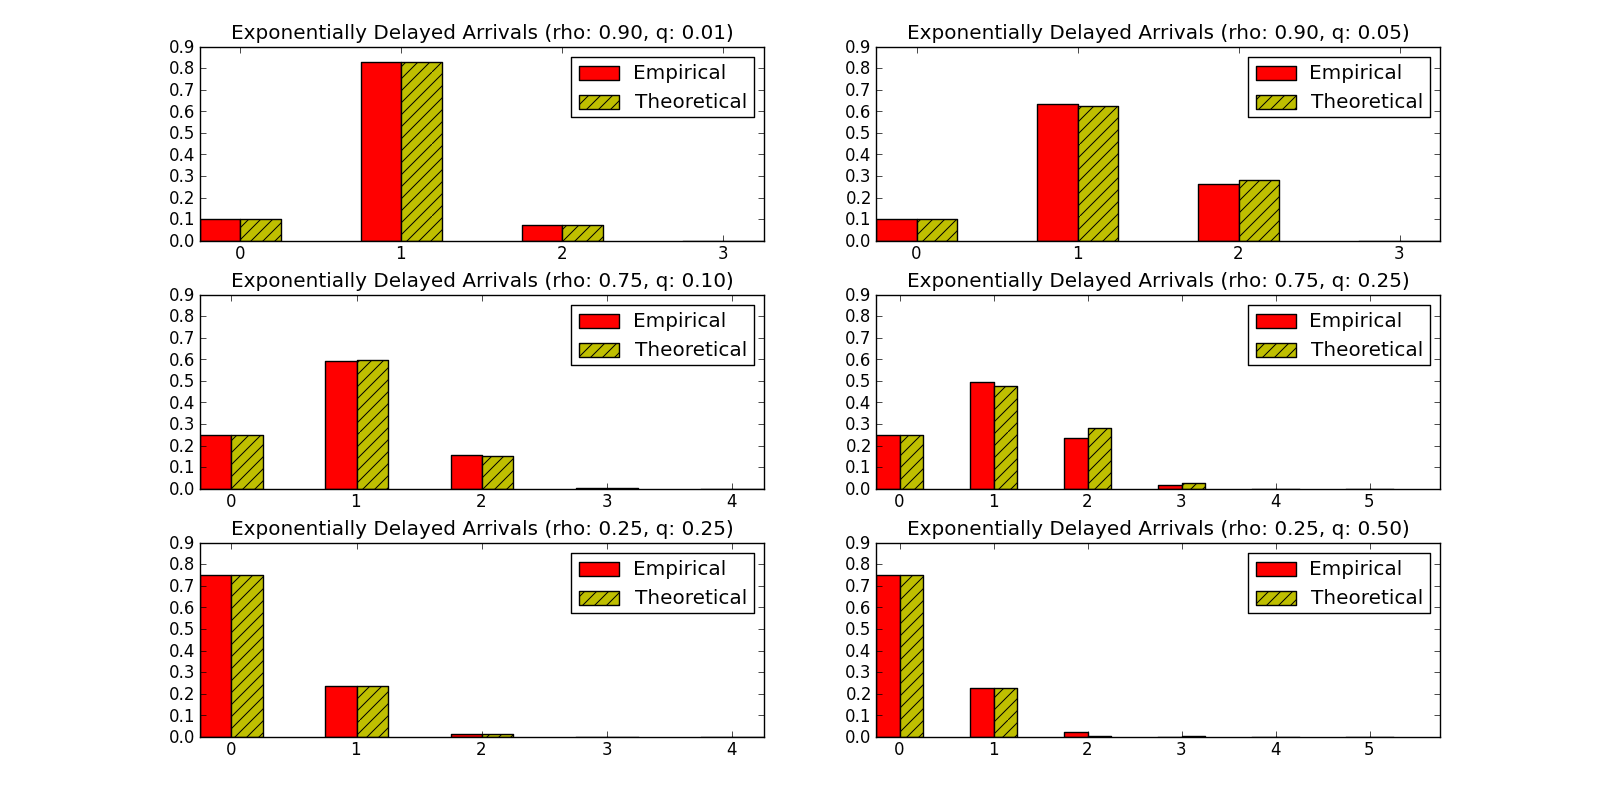
\includegraphics[width=.9\textwidth]{compare}
\end{frame}

\begin{frame}[t]\frametitle{The marginal distribution of late customers}
    If we evaluate in $z=1$ the expression
    \[P(z,y)= \frac{1 - \rho + \rho(z+q(y-z))}{z}\Big[ (z-1)P(0,z+q(y-z))
    + P(z, z+q(y-z))\Big]\,,\]
    we get
    \[P(1,y) = [1 - \rho + \rho q (1-y)] \, P(1, 1 + q(1-y))\]
    Iterating yields
    \[P(1,y) = \sum_l y^l \sum_n P_{n,l} = \prod_{k\geq1}(1+\rho q^k(y-1))\,.\]

    \begin{alertblock}{Remarks}
        \begin{itemize}
            \item $P(1,y) = \frac{(\rho(1-y);q)_\infty}{1+\rho(y-1)}$
            \item $(a;q)_\infty$ is the infinite \emph{$q$-Pochhammer symbol},
            aka $q$-ascending factorial in $a$
        \end{itemize}
    \end{alertblock}
\end{frame}

\begin{frame}[t]\frametitle{The marginal distribution of late customers}
    \begin{theorem}[Lancia et al, 2017]
        The marginal distribution of the number of late customers satisfies
        \begin{equation*}
            \sum_n P_{n,l}= \sum_{k\geq l} (-1)^{k-l}\rho^k\,q^{\binom{k+1}{2}} \,\binom{k}{l} \left[1+\prod_{i=1}^k\frac{1}{1-q^i}\right].
        \end{equation*}
    \end{theorem}
    \begin{itemize}
        \item The marginal distribution decays super-exponentially fast in $l$.
        \item The factor $1+\prod_{i=1}^k\frac{1}{1-q^i}$ is the
        generating function of the number of partitions into at most $k$
        parts;
        \item The problem shows a rich combinatorial structure.
    \end{itemize}
\end{frame}

\begin{frame}[t]\frametitle{Asymptotic result}
    \begin{itemize}
        \item $\sum_n P_{n,l} = O(\rho^l\,q^{\binom{l+1}{2}})$
        \item Let $\alpha_t = n_t + l_t$
        \item The generating function of the equilibrium distribution of $\alpha_t$ is
        \[\sum_{a} \sum_{n+l=a} P_{n,l} z^{a} = \sum_{n+l} P_{n,l} z^{n+l} = P(z,z)\]
    \end{itemize}
    Since
    \[\sum_{n+l=a} P_{n,l} = \frac{1}{a!} \frac{d^a}{dz^a}P(z,z) = P_{0,a} + \frac{\rho}{1-\rho}P_{0,a-1}\,,\]
    \begin{theorem}[Lancia et al, 2017]
        For $a = n+l$,
        \[P_{n,l} = O(\rho^a\,q^{\binom{a}{2}})\]
    \end{theorem}
\end{frame}

\begin{frame}[t]\frametitle{Approximation scheme}
    \begin{columns}
        \column{.5\textwidth}
        \begin{itemize}
            \item We truncate the infinite system of balance equations
            \item Fix an integer $\alpha_{\text{max}}$
            \item Impose $P_{n,l} = 0$ for $n + l > \alpha_{\text{max}}$
        \end{itemize}
        \column{.5\textwidth}
        \centering
        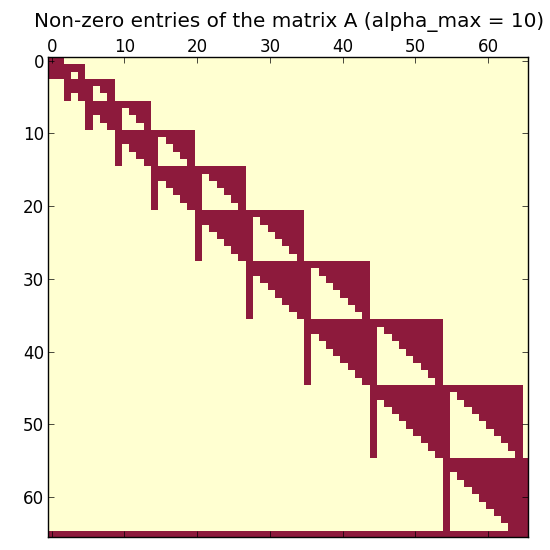
\includegraphics[width=.75\textwidth]{spyAbar}
    \end{columns}
\end{frame}

\begin{frame}[t]\frametitle{A priori bound}
    \begin{columns}
        \column{.5\textwidth}
        \begin{itemize}
            \item From perturbation theory
            \[\sum_{n,l < \alpha_{\text{max}}} | P_{n,l} − \tilde{P}_{n,l} | \leq  \kappa(A) \epsilon_{n,l}\]
            \item $\epsilon_{n,l}$ can be uniformly bounded by $\frac{(-q;q)_\infty}{(q;q)_\infty}q^{\binom{\alpha_{\text{max}}}{2}}$
            \item $\kappa(A) = \Vert A \Vert_1 \Vert A^{-1} \Vert_1$ is the condition number of the truncated matrix $A$
            \item Plot of the uniform bound for $\alpha_{\text{max}}= 100$
        \end{itemize}
        \column{.5\textwidth}
        \centering
        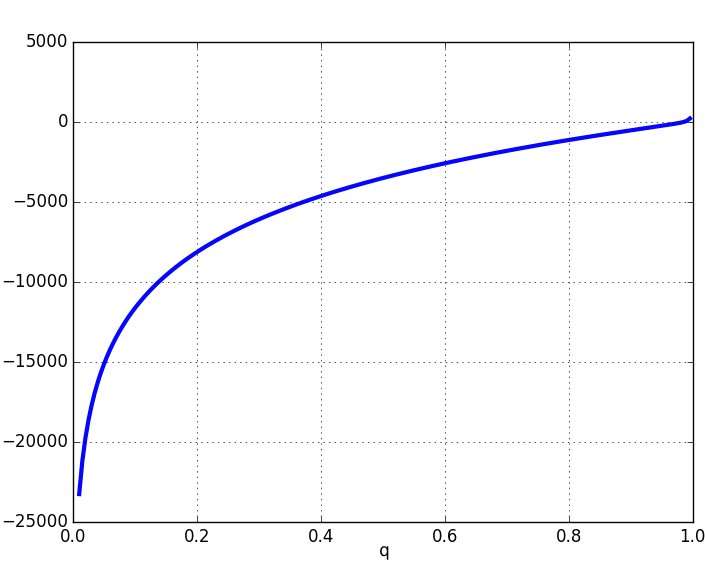
\includegraphics[width=.75\textwidth]{logBound1}
    \end{columns}
\end{frame}

\begin{frame}[t]\frametitle{A priori bound}
    \begin{columns}
        \column{.5\textwidth}
        \begin{itemize}
            \item From perturbation theory
            \[\sum_{n,l < \alpha_{\text{max}}} | P_{n,l} − \tilde{P}_{n,l} | \leq  \kappa(A) \epsilon_{n,l}\]
            \item $\epsilon_{n,l}$ can be uniformly bounded by $\frac{(-q;q)_\infty}{(q;q)_\infty}q^{\binom{\alpha_{\text{max}}}{2}}$
            \item $\kappa(A) = \Vert A \Vert_1 \Vert A^{-1} \Vert_1$ is the condition number of the truncated matrix $A$
            \item Plot of the condition number for $\alpha_{\text{max}}= 100$
        \end{itemize}
        \column{.5\textwidth}
        \centering
        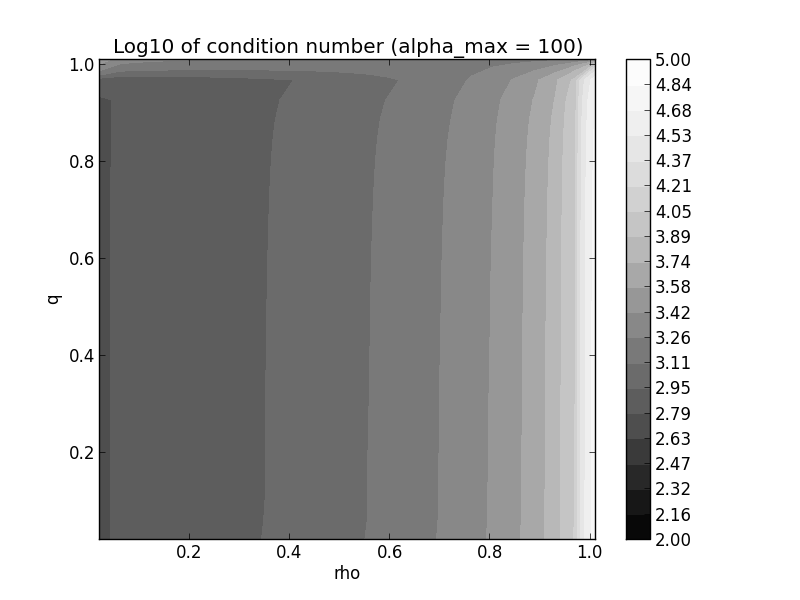
\includegraphics[width=.95\textwidth]{CondNo_alpha_100}
    \end{columns}
\end{frame}


\begin{frame}{Conclusions}
    \begin{itemize}
        \item PSRA describes better the inbound flow than Poisson arrivals
        \item Poisson arrivals lead to \alert{overestimation of the queue}
        \item Only advantage of Poisson is mathematical tractability
        \item If time scale is small, \alert{only the transient matters, \emph{i.e. no benefit}}
        \item PSRA are difficult to tackle, even in the \emph{simple} case of EDA
        \item Efficient approximation schemes are possible, see Guadagni et al 2011
    \end{itemize}

    \begin{alertblock}{Acknowlegments}
        Lorenzo Capanna and Luigi De Giovanni for querying the DDR database
    \end{alertblock}

    \begin{alertblock}{Preprints}
        \begin{itemize}
            \item Lancia et al (2017) \url{https://arxiv.org/abs/1302.1999}
            \item Lancia, Lulli (2017) \url{https://arxiv.org/abs/1708.02486}
        \end{itemize}
    \end{alertblock}
\end{frame}


\end{document}
